\documentclass[10pt]{article}
\usepackage[letterpaper]{geometry}
\geometry{verbose,tmargin=1in,bmargin=1in,lmargin=1in,rmargin=1in}
\usepackage{setspace}
\usepackage{ragged2e}
\usepackage{algorithm2e,etoolbox}
\AtBeginEnvironment{algorithm}{\let\textnormal\ttfamily\DontPrintSemicolon}
\usepackage{color, colortbl}
\usepackage{titlesec}
\usepackage{graphicx}
\usepackage{float}
\usepackage{mathtools}
\usepackage{amsmath}
\usepackage[font=small,labelfont=bf,labelsep=period]{caption}
\usepackage[english]{babel}
\usepackage{indentfirst}
\usepackage{array}
\usepackage{makecell}
\usepackage[usenames,dvipsnames]{xcolor}
\usepackage{multirow}
\usepackage{tabularx}
\usepackage{arydshln}
\usepackage{caption}
\usepackage{subcaption}
\usepackage{xfrac}
\usepackage{etoolbox}
\usepackage{cite}
\usepackage{url}
\usepackage{dcolumn}
\usepackage{hyperref}
\usepackage{courier}
\usepackage{url}
\usepackage{esvect}
\usepackage{commath}
\usepackage{verbatim} % for block comments
\usepackage{enumitem}
\usepackage{hyperref} % for clickable table of contents
\usepackage{braket}
\usepackage{titlesec}
\usepackage{booktabs}
\usepackage{gensymb}
\usepackage{longtable}
\usepackage{glossaries}
\usepackage{tcolorbox} % for colored boxes
\tcbuselibrary{breakable} % to allow colored boxed to extend over multiple pages
\usepackage[mathscr]{euscript} % for script letters
\usepackage{wasysym}  % for checkboxes
\usepackage{bm} % for bolding math symbols
\usepackage{listings} % for including code in boxes
\setcounter{MaxMatrixCols}{20} % sets max matrix length as 20 columns

\lstdefinestyle{mystyle}{ 
    commentstyle=\color{gray},
    keywordstyle=\color{magenta},
    stringstyle=\color{orange},
    basicstyle=\footnotesize,
    language=C++,
    breakatwhitespace=false,         
    breaklines=true,                 
    captionpos=b,                    
    keepspaces=true,                 
    numbers=left,                    
    numbersep=5pt,                  
    showspaces=false,                
    showstringspaces=false,
    showtabs=false,          
    basicstyle=\small\ttfamily,        
    tabsize=2
}

\lstset{style=mystyle}

% change spacing around sections
\titlespacing*{\section}
{0pt}{10ex}{1ex}
\titlespacing*{\subsection}
{0pt}{7ex}{1ex}

% new commands for shorter writing of equations
\newcommand{\beq}{\begin{equation}}
\newcommand{\eeq}{\end{equation}}
\newcommand{\beqa}{\begin{equation}\begin{aligned}}
\newcommand{\eeqa}{\end{aligned}\end{equation}}

% Acronyms used
\setacronymstyle{long-short}
\newacronym{anl}{ANL}{Argonne National Laboratory}
\newacronym{cfd}{CFD}{Computational Fluid Dynamics}
\newacronym{fe}{FE}{Finite Element}
\newacronym{fem}{FEM}{Finite Element Method}
\newacronym{inl}{INL}{Idaho National Laboratory}
\newacronym{io}{I/O}{Input/Output}
\newacronym{moon}{MOON}{MOOSE and Nek}
\newacronym{moose}{MOOSE}{the Multiphysics Object-Oriented Simulation Environment}

\titleclass{\subsubsubsection}{straight}[\subsection]

% define new command for triple sub sections
\newcounter{subsubsubsection}[subsubsection]
\renewcommand\thesubsubsubsection{\thesubsubsection.\arabic{subsubsubsection}}
\renewcommand\theparagraph{\thesubsubsubsection.\arabic{paragraph}} % optional; useful if paragraphs are to be numbered

\titleformat{\subsubsubsection}
  {\normalfont\normalsize\bfseries}{\thesubsubsubsection}{1em}{}
\titlespacing*{\subsubsubsection}
{0pt}{3.25ex plus 1ex minus .2ex}{1.5ex plus .2ex}

\makeatletter
\renewcommand\paragraph{\@startsection{paragraph}{5}{\z@}%
  {3.25ex \@plus1ex \@minus.2ex}%
  {-1em}%
  {\normalfont\normalsize\bfseries}}
\renewcommand\subparagraph{\@startsection{subparagraph}{6}{\parindent}%
  {3.25ex \@plus1ex \@minus .2ex}%
  {-1em}%
  {\normalfont\normalsize\bfseries}}
\def\toclevel@subsubsubsection{4}
\def\toclevel@paragraph{5}
\def\toclevel@paragraph{6}
\def\l@subsubsubsection{\@dottedtocline{4}{7em}{4em}}
\def\l@paragraph{\@dottedtocline{5}{10em}{5em}}
\def\l@subparagraph{\@dottedtocline{6}{14em}{6em}}
\makeatother

\newcommand{\volume}{\mathop{\ooalign{\hfil$V$\hfil\cr\kern0.08em--\hfil\cr}}\nolimits}

\numberwithin{equation}{section} % for equation numbering

\setcounter{secnumdepth}{4}
\setcounter{tocdepth}{4}
\makeglossaries
\begin{document}

\title{OpenMC, BISON, and Nek Coupling}
\author{Argonne National Laboratory}
\maketitle

\tableofcontents
%\printglossary[type=\acronymtype,title=Abbreviations]

\clearpage

\section{Introduction}

This document is intended to describe the coupling methodology between Nek, a \gls{cfd} code developed by \gls{anl}, OpenMC, a Monte Carlo code developed by \gls{anl}, and BISON, a nuclear fuel performance code developed by \gls{inl}. Previous work by Matthew Ellis and others at MIT resulted in the coupling of OpenMC to MOOSE, and work by a joint effort of \gls{anl} and \gls{inl} resulted in the coupling of Nek to MOOSE. So, the coupling of all three codes together will attempt to utilize as much as possible regarding this previous work. The purpose of this report is to document the coupling process, justify decisions made, and illustrate how to use these codes in a coupled manner.

This report is organized beginning with a description of the overall coupling methodology, followed by a discussion of the nuts-and-bolts requirements for coupling two codes in terms of the data transfer between the codes and executing non-MOOSE codes from within the MOOSE framework.

\section{Overall Coupling Methodology}
This section discusses the overall coupling methodology that was pursued between OpenMC-BISON, BISON-Nek, and finally OpenMC-BISON-Nek. The immediate jump to the coupling of all three codes together was not performed because taking smaller steps often helps reveal difficulties that would otherwise be compounded and confusing when performing the full three-way coupling. 

When coupling two or more distinct projects (code bases), there are generally three ways to perform the coupling:

\begin{enumerate}
\item Make virtually no changes to the source code of the two projects, and instead write an external script that will:
	\begin{enumerate}
	\item Run the first code.
	\item Read the text output file of the first code and modify the text input file for the second code.
	\item Run the second code.
	\item Read the text output file of the second code and modify the text input file for the first code. 
	\item Repeat (a)-(d) until convergence, then move to the next time step.
	\end{enumerate}
	This approach is necessary for proprietary codes for which you have no access to the source code, and the only interaction with the software is through text files.
\item Write a custom driver that will call routines from each code. This may be fast to develop, but limits the reusability of the driver itself or changes made to the two codes to meld to the driver structure. For example, pseudo-code for a driver written to couple OpenMC and Nek may have the following overall structure:

	\begin{algorithm}[H]
	{\tt initialize OpenMC}\;
	{\tt initialize Nek}\;
	\;
	\While{t $<$ end time}{
	  \While{not converged}{
	    run OpenMC\;
	    transfer data to Nek\;
	    run Nek\;
	    transfer data to OpenMC\;
	    evaluate convergence\;
	  }
	}
	\end{algorithm}
	
\item Use an existing driver with a sufficiently general structure that the codes you want to couple can be structurally modified to be callable from within the existing driver by directly calling code routines (no editing of text files). This approach, by virtue of using an existing driver, allows you to immediately take advantage of the ability to couple to any other codes that have been cast in terms of the existing driver's methods. However, this approach requires a good understanding of the existing driver, which can be much more time consuming than developing a custom driver from scratch. In addition, the downsides of using an existing coupling framework include potentially less control over parallelism and performance, since applications must be mapped to the structure of the existing driver, which may not be ideal for every application.
\end{enumerate}

The third approach of using an existing driver framework was selected for this work given the reasons above. More specifically, the MOOSE framework was selected for the following reasons:

\begin{enumerate}
\item Many applications have been developed with the MOOSE framework, such as nuclear fuels simulations (BISON), porous media thermal-hydraulics (PRONGHORN), radiation damage and structural modeling (GRIZZLY), and many other physics. Using the MOOSE coupling framework allows OpenMC and Nek to essentially become "MOOSE" Animals in that they can not only be coupled to each other, as the scope of this project seeks, but to these other codes with relatively minor effort.
\item Significant work has already been performed with coupling OpenMC to MOOSE and Nek to MOOSE, so the coupling of OpenMC with Nek in principle can directly take advantage of this existing work.
\item The MOOSE framework is easy-to-use and has significant coupling capabilities already developed, as well as an accessible development team for assistance.
\end{enumerate}

If the parallel performance is not acceptable, then the work developed in constructing OpenMC and Nek as MOOSE applications can still be reused for a custom driver due to MOOSE's modular structure. The MOOSE coupling framework performs coupling in a tree-like structure. A Master App controls the entire coupled solver, and is the App that performs actions such as initializing MPI. For the Master App, there may be any number of sub-applications. The terminology "Sub-app" and "MultiApp" are essentially the same, where the use of sub app is used primarily to denote that a MultiApp is "down-the-tree" from another MultiApp. 

\begin{figure}[H]
\centering
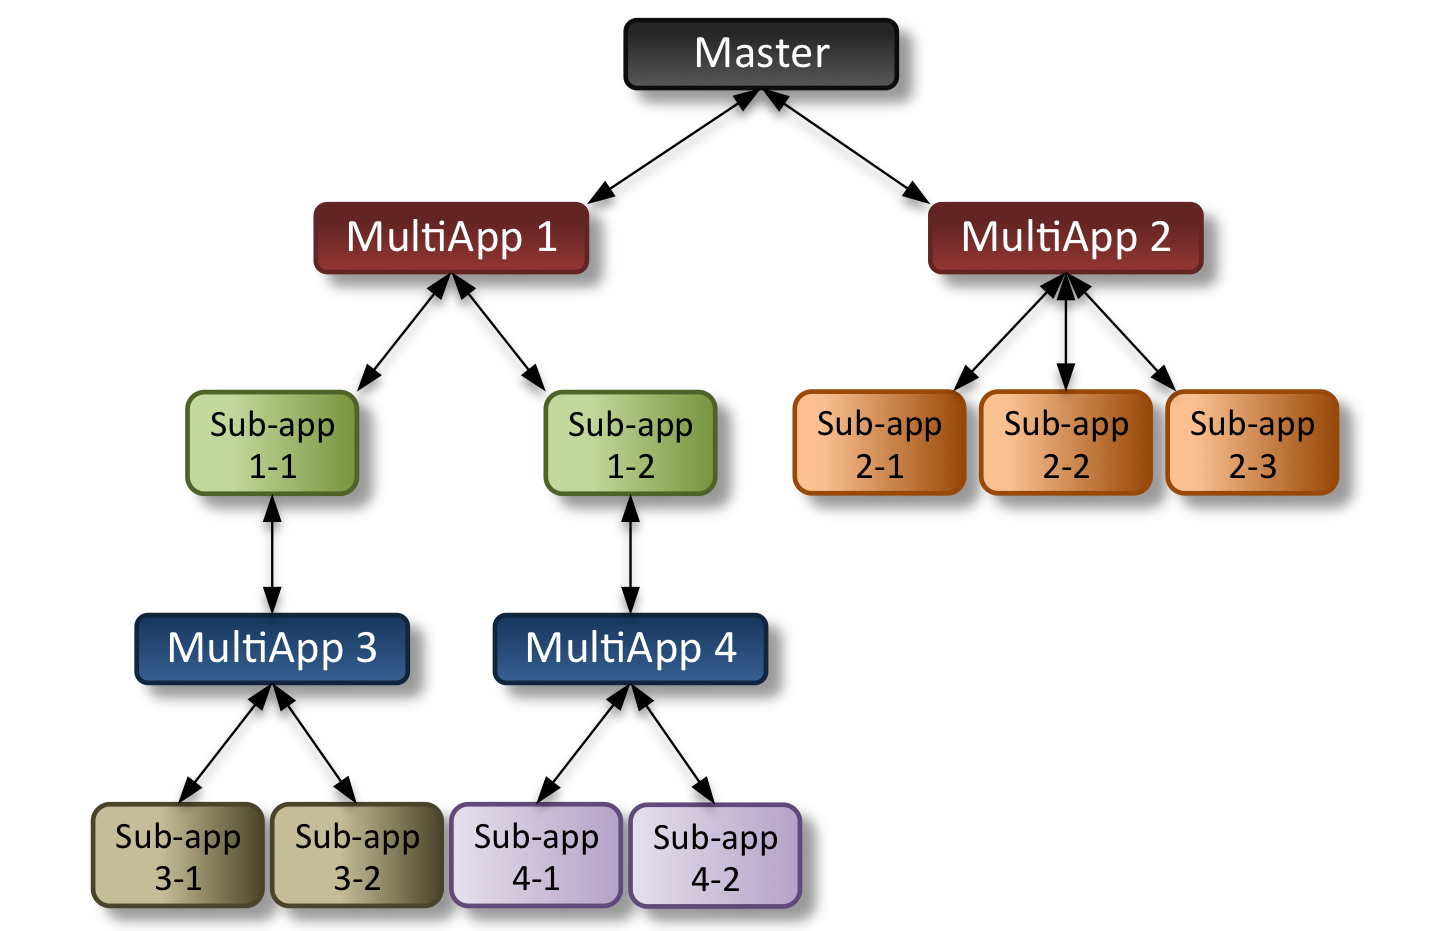
\includegraphics[width=10cm]{multiapp_hierarchy.png}
\caption{MasterApp and MultiApp structure for a MOOSE simulation.}
\end{figure}

The Master App coordinates the main solve, and will call the execution methods of its immediate MultiApps when needed. Those immediate MultiApps may have their own MultiApps, and hence act somewhat locally as Master Apps. 

The remainder of this section discusses the high-level coupling strategy for OpenMC-MOOSE, Nek-MOOSE, and finally OpenMC-Nek-BISON. 

\subsection{OpenMC and BISON Coupling}
This section discusses the OpenMC-BISON coupling, illustrated through a pair of specific example input files that can be found in {\tt okapimcs/tests/FETs/bison-openmc}. For the most generic OpenMC-BISON coupling, MOOSE is the Master App, and OpenMC is wrapped as a MOOSE App so that it can be called as a MultiApp to the MOOSE Master App. BISON is already a MOOSE animal, and hence does not require any wrapping. So, for this coupling scheme, MOOSE is the Master App, and Okapi and BISON are same-level MultiApps. In a coupled solve, the following steps occur. We arbitrarily choose OpenMC to execute before BISON, so we choose to execute OpenMC on {\tt timestep\_begin}, and BISON on {\tt timestep\_end}. 

\begin{enumerate}
\item Initialize the MasterApp. The MasterApp does not perform any solves, but only exists to transfer data between its MultiApps.
\item Initialize OpenMC. This calls the {\tt OpenMCExecutioner::init()} method, which performs the regular initialization steps for any MOOSE App, followed by calling the {\tt openmc\_init} subroutine found in the OpenMC source. This subroutine performs basic tasks such as reading in the XML files that control OpenMC parameters (none are set in the MOOSE input files), allocating memory for data structures, etc.
\item Initialize BISON. Because BISON is a Moose ``animal,'' this simply calls initialization method of the MOOSE executioner that we chose to use (for most cases, this will be {\tt Transient::init()}).
\item Perform any transfers that are defined on {\tt timestep\_begin} to the MultiApps. 
	\begin{enumerate}
	\item This calls the {\tt PolynomialOpenMC::execute()} method to pass the {\tt l\_0\_coeffs\_temp} scalar variable to OpenMC. Because OpenMC is not a MOOSE ``animal,'' we cannot simply use the {\tt MultiAppScalarToAuxScalarTransfer}. For this step, we are transferring from MOOSE to Okapi, so we call the {\tt OpenMC::openmc\_cell\_set\_temperature} method, which takes as its arguments the OpenMC cell to change temperature and a single value. Without continuous material tracking implemented yet in OpenMC, this only selects the first expansion coefficient for temperature (so this transfer is incomplete). This is where an initial condition on temperature is applied in OpenMC.
	\end{enumerate}
\item Execute OpenMC by calling the {\tt OpenMCExecutioner::execute()} method, which calls the {\tt openmc\_reset} and {\tt openmc\_run} subroutines in the OpenMC source. This performs a full Monte Carlo solve.
\item Transfer information back from OpenMC to the MOOSE Master App. This is done by calling the {\tt PolynomialOpenMC::execute} method, for a direction from OpenMC to a Master App. This method then calls the {\tt fet\_deconstruction} subroutine in the OpenMC source, which stores the expansion coefficients for the FETs (which we indicated in the tallies XML input) by cell index. Then, the {\tt get\_coeffs\_from\_cell} subroutine is called to store the expansion coefficients in OpenMC in a C++ array. Finally, those values are stored in the {\tt l\_0\_coeffs\_power} scalar variable in the MOOSE Master App.
\item ``Solve'' the Master App. This is purely a dummy solve, but is required for any auxkernels to evaluate, and for any further transfers to occur.
\item Transfer information from the MOOSE Master App to BISON. This uses the {\tt MultiAppScalarToAuxScalarTransfer} to simply copy the coefficients for power held in {\tt l\_0\_coeffs\_power} to the {\tt l\_0\_coeffs\_power\_bison} variable in BISON.
\item BISON uses these coefficients to expand a continuous field variable {\tt bison\_kappa\_fission}, which holds the kappa fission distribution that was calculated by OpenMC. Functions for the Legendre, Zernike, and reconstruction are included in the BISON input file.
\item BISON then applies the {\tt KappaFissionToHeatSource} auxkernel on the {\tt bison\_heat} auxvariable to convert the kappa fission source to the correct units of W/volume that is used as a heat source in the {\tt HeatSource} kernel.
\item Solve BISON to solve for the temperature, {\tt bison\_temp}.
\item BISON deconstructs this continuous temperature field into a set of expansion coefficients, stored in {\tt l\_0\_coeffs\_temp\_bison} by calling the {\tt ZLDeconstruction} user object.
\item Transfer coefficients for temperature from BISON to MOOSE by calling the {\tt MultiAppScalarToAuxScalarTransfer} transfer. These coefficients are stored in the {\tt l\_0\_coeffs\_temp} variable in MOOSE. 
\item Repeat steps 4-13 for each Picard step until reaching the end of the coupled simulation.
\end{enumerate}

To summarize the above detailed steps, the following graphic shows the generic data flow for a single Picard step (i.e. the first three steps of initializing the Master App and two MultiApps are assumed to have occurred). Individual steps are numbered in the order in which they occur.

\begin{figure}[H]
\centering
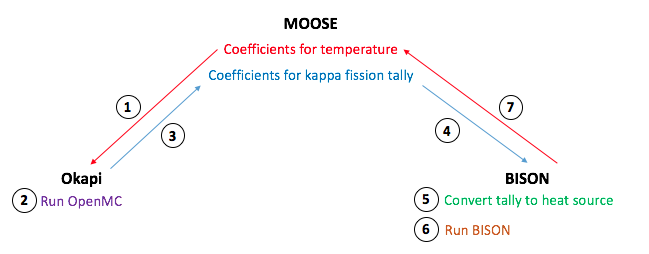
\includegraphics[width=15cm]{OpenMC-BISON-simple.png}
\end{figure}

And, in more detail, the following figure provides the names of the methods that are called to perform each step and shows the deconstruction and reconstruction actions in BISON.

\begin{figure}[H]
\centering
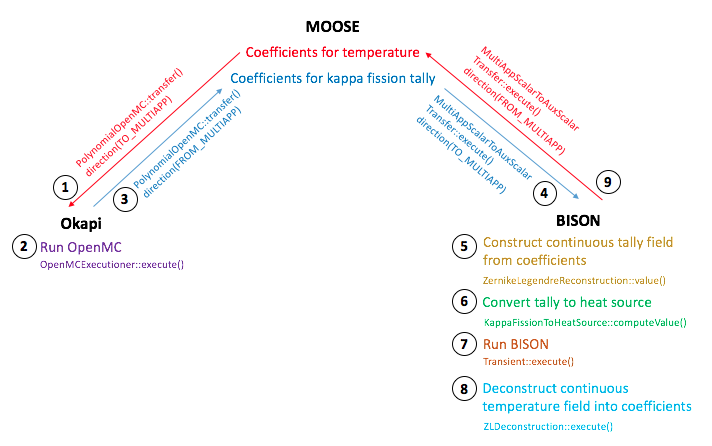
\includegraphics[width=15cm]{OpenMC-BISON-complicated.png}
\end{figure}

\section{Data Transfer}

This section discusses the requirements needed to transfer information between two physics codes. When coupling two codes, there are two general ways in which the data can be transferred:

\begin{enumerate}
\item Force both codes to solve on the same mesh, in which case the data transfer can be accomplished by determining a functional form for the transfer variable (such as temperature) over a single computational element, and then passing this information to the second code. Assuming that the second code can utilize this information exactly, this is the easiest way to transfer information, because it requires little effort to map cells in one mesh to cells in another. However, this method is very restrictive, since it is often the case that the two physics do not require the same mesh, and forcing both physics to run on the finest mesh is unnecessarily expensive. For instance, boundary layers must be resolved for fluids computations with very fine elements that would be overkill for a Monte Carlo simulation.
\item Run both codes on different meshes.

	\begin{enumerate}
	\item Use arbitrary polynomials to express a transfer variable, and then pass the expansion coefficients to the second code. For instance, suppose Nek is to transfer temperature on a boundary to MOOSE, which would use this information to set a boundary condition. Because this information is not being passed on an element-to-element basis, its spatial distribution must be described using some type of function - delta functions if an elementwise-constant value from Nek is to be transferred to an element (not necessarily of the same size) in MOOSE, or really any arbitrary polynomial. To transfer a variable \(u(r, \theta, z)\) to MOOSE, Nek would compute the expansion coefficients \(C_{jkl}\) that capture the behavior according to expansion functions \(R(r), \Theta(\theta), Z(z)\):
	
	\beq
	\label{eq:GenericExpansion}
	u(r, \theta, z)\approx\sum_{j=0}^J\sum_{k=0}^K\sum_{l=0}^L C_{jkl}R_j(r)\Theta_k(\theta)Z_l(z)
	\eeq
	
Note that an approximate equals sign \(\approx\) is used, since for an arbitrary selection of functions, the (potentially) infinite degrees of freedom of the value of \(u\) computed by Nek cannot be fully captured. Once Nek passes the coefficients \(C_{jkl}\) to MOOSE, MOOSE would reconstruct the functional form of the transfer variable using the same equation above, and then proceed with its simulation for that step. The issue with using arbitrary polynomials is that there is no one way to determine the expansion coefficients \(C_{jk}\). For instance, assume we use the following expansion functions:

	\beqa
	R_j(r)=&r^j\\
	\Theta_k(\theta)=&\cos(k\theta)\\
	Z_l(z)=&1+z^l\\
	\eeqa

To determine the expansion coefficients for this choice requires that we construct a Vandermonde matrix, which requires that we arbitrarily select points over the Nek element at which to sample the Nek transfer variable. For \(J=1\), \(K=0\), \(L=0\), this matrix system would take the form:

\beqa
u(r,\theta,z)=\begin{bmatrix}
r_0^0\cos{(0)}(1+z_0^0) & r_0^1\cos{(\theta_0)}(1+z_0^0)\\
r_1^0\cos{(0)}(1+z_0^0) & r_1^1\cos{(\theta_0)}(1+z_0^0)\\
\end{bmatrix}
\begin{bmatrix}
C_{000}\\C_{100}
\end{bmatrix}
\eeqa

where \(r_0\) and \(r_1\) are the two sampled \(r\)-coordinates in the element that must be selected in order to determine the expansion coefficients for a first-order \(r\)-expansion, and \(\theta_0\) and \(z_0\) the sampling points to determine the expansion coefficients for a zeroth-order \(\theta\)- and \(z\)-expansion. This can cause problems such as oscillations in the interpolation if the choices of functions are poor, and can completely miss parts of the transfer variable solution if we happen to not select points near important features.

	\item Use orthogonal functions to express a transfer variable, and then pass the expansion coefficients to the second code. Using orthogonal functions is essentially the same formulation as that shown in Eq. \eqref{eq:GenericExpansion}, except that the expansion functions are chosen to be orthogonal over the domain of transfer. Then, orthogonality conditions lead to exact formulas for \(C_{jkl}\) that are {\it integral} in nature, which means that all features of the solution are captured, and no creation and inversion of a Vandermonde matrix is required. 
	\end{enumerate}
	
\end{enumerate}

For the reasons discussed above, the data transfer between two physics codes can be performed in a fairly simple manner when using orthogonal polynomial expansions. This is the approach that is taken in the coupling of Nek, OpenMC, and BISON, and therefore warrants more discussion. For any code to implement data transfers using polynomials, four capabilities are required:

\begin{enumerate}
\item Functions to compute the orthogonal polynomials given a coordinate point and expansion order.
\item Routines to integrate a continuous variable over an orthogonal domain to compute the expansion coefficients. This process will be referred to in this document as ``deconstruction,'' since a continuous field is decomposed into a finite set of expansion coefficients that are to be passed to another physics code.
\item Routines to multiply a set of expansion coefficients by orthogonal polynomials to form a continuous field form a set of finite coefficients. This process will be referred to in this document as ``construction,'' since a continuous field is formed by multiplying discrete expansion coefficients by continuous functions.
\item Use the constructed field in some internal capacity that defines the coupling, such as in the specification of a boundary condition or heat source.
\end{enumerate}

For the three physics codes to be discussed, each of these four capabilities will be described in detail.

\subsection{Choices of Orthogonal Polynomials}
\label{sec:Polynomials}
This section describes several choices of orthogonal polynomials that can be used to construct and deconstruct continuous fields.

\subsubsection{Legendre Polynomials}

Legendre polynomials are orthogonal over \( -1 \leq z \leq 1\), and hence are suitable for expanding solutions along the axes of fuel pins, along one direction in a slab, or in any Cartesian dimension. The Legendre polynomials are given as:

\beq
\label{eq:Legendre}
P_l(z)=\frac{1}{2^ll!}\frac{d^l}{dx^l}\left\lbrack\left(z^2-1)^l\right)\right\rbrack
\eeq

which are orthogonal over \(-1\) to \(+1\):

\beq
\int_{-1}^{+1}P_l(z)P_{l'}(z)dz=\frac{2}{2l+1}\delta_{ll'}
\eeq

When calculating expansion coefficients, it will be useful to work with scaled Legendre polynomials such that the orthogonality condition gives {\it only} a delta function. These scaled Legendre polynomials are indicated with a tilde:

\beq
\label{eq:LegendreScaled}
\tilde{P}_l(z)=\sqrt{\frac{2l+1}{2}}P_l(z)
\eeq

such that the orthogonality condition becomes:

\beq
\label{eq:LegendreScaledOrthogonality}
\int_{-1}^{+1}\tilde{P}_l(z)\tilde{P}_{l'}(z)dz=\delta_{ll'}
\eeq

\subsubsection{Fourier Polynomials}

Fourier polynomials are orthogonal over \(-\pi\leq\theta\leq\pi\), and hence are suitable for expanding along the \(\theta\) direction of a cylindrical fuel pin. The Fourier functions are given as:

\beq
\label{eq:Fourier}
F_k(\theta)=\cos(k\theta)
\eeq

which are orthogonal over \(-\pi\) to \(+\pi\):

\beqa
\label{eq:FourierOrthogonal}
\begin{cases}
\int_{-\pi}^{+\pi}F_k(\theta)F_{k'}(\theta)d\theta=2\pi\delta_{kk'}& k=k'=0\\
\int_{-\pi}^{+\pi}F_k(\theta)F_{k'}(\theta)d\theta=\pi\delta_{kk'}& \textrm{else}\\
\end{cases}
\eeqa

and hence for \(n=0\), the return value is scaled by \(1/\sqrt{2\pi}\) instead of \(1/\sqrt{\pi}\). 

Similar to Legendre polynomials, it will be more convenient when calculating expansion coefficients for the Fourier polynomials to be scaled such that the orthogonality condition gives {\it only} a delta function. These scaled Fourier polynomials are indicated with a tilde:

\beq
\label{eq:FourierScaled}
\tilde{F}_k(\theta)=\frac{1}{\sqrt{\pi}}\cos{(k\theta)}
\eeq

such that the orthogonality condition becomes:

\beq
\int_{-\pi}^{+\pi}\tilde{F}_k(\theta)\tilde{F}_{k'}(\theta)d\theta=\delta_{kk'}
\eeq

\subsubsection{Zernike Polynomials}

Zernike polynomials are orthogonal over the unit circle, and hence are suitable for expanding in the plane of a fuel pin. The Zernike polynomials are given as:

\beq
\label{eq:ZernikeScaled}
Z_n^m(r,\theta)=
\begin{cases}
\sqrt{\frac{2(n+1)}{\pi\left(1+\delta_{m0}\right)}}R_n^{|m|}(r)\cos{(m\theta)} & m\geq 0\\
-\sqrt{\frac{2(n+1)}{\pi\left(1+\delta_{m0}\right)}}R_n^{|m|}(r)\sin{(m\theta)} & m < 0\\
\end{cases}
\eeq

where \(R_n^{|m|}\) is given as:

\beq
R_n^{|m|}(r)=\sum_{s=0}^{\frac{n-|m|}{2}}\frac{(-1)^s(n-s)!}{s!\left(\frac{n+|m|}{2}-s\right)!\left(\frac{n-|m|}{2}-s\right)!}r^{n-2s}
\eeq

Note that \(m\) can only obtain values \(-n, -n+2, -n+4, \cdots, n\). For this definition of the Zernike polynomials, which include the normalization factor that was similarly introduced for Fourier and Legendre polynomials, the orthogonality condition over the unit circle reads:

\beq
\label{eq:ZernikeOrthogonal}
\int_{0}^{1}rdr\int_{0}^{2\pi}d\theta Z_{n}^m(r,\theta)Z_{n'}^{m'}=\delta_{n,n'}\delta_{m,m'}
\eeq

\subsection{Deconstructing a Continuous Variable}
This section describes how a continuous field \(u(r,\theta,z)\) can be deconstructed into a set of expansion coefficients using the orthogonal polynomials discussed in the previous section. The procedure is the same regardless of the orthogonal domain (i.e. if performing a boundary or volume coupling), but will be illustrated for both a boundary coupling over the surface of a cylinder and for a volume coupling over a cylindrical domain. 

For a boundary coupling over the surface of a cylinder, a function \(u(\theta,z)\) can be expressed as:

\beq
\label{eq:OrthogonalExpansion}
u(\theta, z)\approx\sum_{k=0}^K\sum_{l=0}^LC_{kl}\tilde{F}_k(\theta)\tilde{P}_l(z)
\eeq

where \(\tilde{F}_k(\theta)\) is the \(k\)-th order Fourier function and \(\tilde{P}_l(z)\) is the \(l\)-th order Legendre polynomial. The expansion coefficients for \(u\) can be determined by multiplying both sides of Eq. \eqref{eq:OrthogonalExpansion} by orthogonal polynomials of different order, and applying the orthogonality conditions given in Section \ref{sec:Polynomials}:

\beq
\label{eq:ScaledExpansionCoeff}
C_{kl}=\int_{-1}^{+1}dz\int_{-\pi}^{+\pi}d\theta u(\theta, z)\tilde{F}_k(\theta)\tilde{P}_l(z)
\eeq

Likewise, for a volume coupling over a cylinder, a function \(u(r,\theta,z)\) can be expressed as:

\beq
\label{eq:ZLReconstruction}
u(r,\theta,z)=\sum_{l=0}^{L}\sum_{n=0}^N\sum_{m=-n}^{n}C_{l}^{nm}\tilde{P}_l(z)\tilde{Z}_n^m(r,\theta)
\eeq

Again, the coefficients can be determined by multiplying by orthogonal polynomials of different order, and applying orthogonality conditions:

\beq
C_l^{nm}=\int_0^1rdr\int_{0}^{2\pi}d\theta\int_{-1}^{1}dzu(r,\theta,z)P_l(z)Z_n^m(r,\theta)
\eeq

Hence, all that is required to deconstruct a continuous field into a set of expansion coefficients is to perform multiple integrations over the orthogonal domain.

\subsection{Constructing a Continuous Variable}

As opposed to deconstruction, constructing a continuous variable from a set of expansion coefficients is more straightforward, since all that is required is repeated evaluation of the orthogonal polynomials, multiplied by expansion coefficients.

\subsection{MOOSE Data Transfer}
This section describes the capabilities introduced into the MOOSE source code that allows evaluation of polynomials, and construction/deconstruction of continuous fields. 

\subsubsection{Evaluation of Polynomials}
This section discusses the generic functions added to MOOSE to compute orthogonal polynomials.

\subsubsubsection{{\tt LegendrePolynomial}}
This function computes the Legendre polynomial in Eq. \eqref{eq:LegendreScaled} for a given value of \(l\) and a specific position (a single value of \(z\)). This function is not particular to the direction in which the Legendre expansion is being made, since only a single number (not a point) is passed in. Because Legendre polynomials are only orthogonal on \([-1, +1]\), but the length of the domain that is being expressed using Legendre polynomials may not necessarily be 2, a scaling factor \(z\) is used to simply stretch or compress the physical domain to the orthogonal domain. The {\tt l\_geom\_norm} required parameter lists the minimum and maximum distances over which the Legendre polynomials will be forced to be orthogonal using a scaling factor. This function exists in both MOON and Okapi, but is cleaner in Okapi.

\subsubsubsection{{\tt FourierPolynomial}}
This function computes the Fourier function given in Eq. \eqref{eq:FourierScaled} for a given value of \(k\) and a specific position. The \(\theta\) value at which to evaluate this function is determined as the angle between the positive \(x\)-axis and a point \((x,y)\). This function is not specific to the direction in which the Legendre expansion is being made, i.e. two points are passed in, where the first is assumed to be the distance along the axis relative to which the angle \(\theta\) is determined. Because the fuel rod of interest for coupling exists on \([-\pi, +\pi]\), no additional scaling is needed like for the Legendre polynomials. This function exists in MOON.

\subsubsubsection{{\tt ZernikePolynomial}}
This function computes a Zernike polynomial given in Eq. \eqref{eq:ZernikeScaled} given orders \(n\) and \(m\). 

\subsubsection{Field Deconstruction}
This section describes how a continuous field is deconstructed into a set of expansion coefficients. 

\subsubsubsection{{\tt NekSideIntegralVariableUserObject}}
This user object determines an expansion coefficient given a field \(u(\theta, z)\) and the orders of the Fourier and Legendre expansions according to Eq. \eqref{eq:ScaledExpansionCoeff}. This user object only computes {\it one} expansion coefficient at a time, and hence for the example shown in the previous section, 50 of these user objects appear in a single input file. Note that this object does not actually compute the integral of \(u(\theta, z)\) - rather, it computes the integral of the heat flux, since this is the variable of interest that is to be expanded in polynomials for transfer to a boundary condition in Nek. This user object is available in MOON.

\begin{lstlisting}
  [./nek_f_4_l_9]
    type = NekSideIntegralVariableUserObject
    variable = temp
    boundary = wall
    legendre_function_name = 'legendre_function'
    fourier_function_name = 'fourier_function'
    l_direction = 2
    l_order = 9
    f_order = 4
    aux_scalar_name = heat_flux_scalar_f_4_l
    diffusion_coefficient_name = 'thermal_conductivity'
    surface_area_pp = 'surf_area'
  [../]
\end{lstlisting}

\subsubsubsection{{\tt ZernikeLegendreDeconstruction}}
This user object converts a continuous variable into the set of expansion coefficients that would be obtained by expanding the variable in Zernike and Legendre polynomials as shown in Eq. \eqref{eq:ZernikeLegendre}. Note that this user object only computes {\it one} \(C_l^{nm}\) at a time. The {\tt ZLDeconstruction} user object should be used instead, since it computes all of the Zernike coefficients given a single Legendre order. Computing each coefficient \(C_{l}^{nm}\) requires applying orthogonality as shown in Eqs. \eqref{eq:ZernikeOrthogonal} and \eqref{eq:LegendreScaledOrthogonality}. Applying both orthogonality conditions to the expansion gives:

\beq
C_l^{nm}=\int_0^1rdr\int_{0}^{2\pi}d\theta\int_{-1}^{1}dzu(r,\theta,z)P_l(z)Z_n^m(r,\theta)
\eeq

In order to determine the correct expansion coefficients, the above integral {\it must} be performed over the integral bounds given, i.e. those over which the functions are orthogonal. However, in the physical domain, the radius of the pin may not be unity, and the \(z\)-extent of the pin may not be from \([-1, 1]\) (though it is assumed that the \(\theta\) coordinate does exist over \([0,2\pi]\)). The integral will be computed in the physical domain. To correctly scale to the orthogonal domain, the integral should be multiplied as follows:

\beq
C_l^{nm}=\frac{1}{R^2}\frac{2}{H}\int_0^1rdr\int_{0}^{2\pi}d\theta\int_{-1}^{1}dzu(r,\theta,z)P_l(z)Z_n^m(r,\theta)
\eeq

where \(R\) is the radius and \(H\) the height in the physical domain. The factor of 2 appears because the height in the orthogonal domain is 2. To prevent the user from needing to enter a radius and height manually, these terms can be found using a postprocessor in MOOSE. By multiplying the factor above by \(\pi/\pi\), the denominator becomes the volume of the region. Hence, a postprocessor value provides the volume.

This user object inherits from the {\tt ElementIntegralUserObject}, which inherits from the {\tt ElementUserObject} class. This parent class inherits all of the parameters of the {\tt BlockRestrictable} interface. Hence, this object can be restricted to blocks using the {\tt blocks} parameter in the XML input file. If the block is not specified, then if a variable parameter is present, the blocks are set to all of the blocks that are associated with that variable (i.e. for most simulations, the entire domain). If no variable is specified, then by default the entire domain is used. 

For a given auxiliary SCALAR variable, the coefficients apply for a fixed Legendre order, and increase in the array beginning with the \(n\) index and then the \(m\) index of the Zernike expansion. The most rigorous way to verify that this deconstruction user object has been implemented correctly is to assume some set of coefficients and reconstruct a polynomial using the {\tt ZernikeLegendreReconstruction} function. Then, deconstruct this function using the {\tt ZernikeLegendreDeconstruction}, and verify that the coefficients have not changed. This must be performed over a cylindrical region to ensure that the orthogonality conditions are true. Note that the coefficients will not perfectly match those specified for the function due to errors associated with the quadrature rule used for numeric integration. This user object is available in Okapi.

\subsubsubsection{{\tt ZLDeconstruction}}
This user object computes {\it all} of the Zernike coefficients given a fixed Legendre order, and hence reduces the number of user objects required in the input file by a factor of the number of Zernike expansion coefficients. The contents of this user object are essentially identical to that of the {\tt ZernikeLegendreDeconstruction} user object, except that loops are used to update an array of values {\tt \_integral\_value}, instead of a singular value.

\subsubsection{Field Reconstruction}
This section discusses the functions developed in MOOSE to reconstruct a continuous field given expansion coefficients and specified orthogonal functions.

\subsubsubsection{{\tt FourierLegendreReconstruction}}
This function reconstructs a solution as a finite series of Fourier and Legendre polynomials given expansion coefficients, and evaluates it at a single point according to Eq. \eqref{eq:OrthogonalExpansion}. While {\tt LegendrePolynomial} and {\tt FourierPolynomial} are {\it not} specific to the orientation of the Legendre expansion relative to any of the Cartesian axes, this reconstruction assumes that given a point with three coordinates, that the third coordinate (the \(z\)-coordinate) serves as input to the {\tt LegendrePolynomial} function, while the \(x\) and \(y\) coordinates are input to the {\tt FourierPolynomial} function. This function is available in MOON.

\begin{comment}
To illustrate how solution reconstruction occurs in MOOSE, consider the following section of a MOON input file. Note that the Legendre and Fourier polynomials are simply instantiated to allow their member {\tt getPolynomialValue} to compute a scalar value given a point (or two for the case of the Fourier polynomial) and an order. The input specifications for {\tt FourierLegendreReconstruction} show that the surface temperature that will be passed from Nek to MOOSE in the form of expansion coefficients will have been expanded in a Legendre order of 10 and a Fourier order of 5. The input to the reconstruction function is a total of {\tt l\_order}\(\times\){\tt f\_order} coefficients. These coefficients are stored in {\tt SCALAR} auxiliary variables. A scalar auxvariable can hold any number of values, and this is implemented as an array of length {\tt ORDER}. For instance, the {\tt temp\_bc\_scalar\_f\_0\_l} auxvariable is declared as {\tt family=SCALAR} and {\tt order=TENTH}, so each of these auxvariables contains 10 scalar values. Each of these variables hence holds the \(C_{0l}, C_{1l}, C_{2l}, C_{3l}, C_{4l}\) values. This helps reduce the total number of variables that must be declared in this input file. For a total of 50 coefficients that are passed back and forth between Nek and MOOSE, this could have been implemented using 50 unique auxvariables, at the expense of a much larger input file.

\begin{lstlisting}
[Functions]
  [./legendre_function]
    type = LegendrePolynomial
    # z-domain exists from 0.0 to 1.0
    l_geom_norm = '0.0 1.0'
  [../]
  [./fourier_function]
    type = FourierPolynomial
  [../]
  [./fl_reconstruction]
    type = FourierLegendreReconstruction
    l_order = 10
    f_order = 5
    # Legendre expansion is for the z-coordinate (not x or y)
    l_direction = 2 
    legendre_function_name = 'legendre_function'
    fourier_function_name = 'fourier_function'
    poly_scalars = 'temp_bc_scalar_f_0_l temp_bc_scalar_f_1_l temp_bc_scalar_f_2_l temp_bc_scalar_f_3_l temp_bc_scalar_f_4_l'
  [../]
[]
\end{lstlisting}

The scalar value returned by the {\tt FourierLegendreReconstruction} function is used in the function Dirichlet boundary condition within MOOSE. 

\begin{lstlisting}
[BCs]
  [./wall]
    type = FunctionDirichletBC
    variable = temp
    boundary = 'wall'
    function = fl_reconstruction
  [../]
[]
\end{lstlisting}

So, this discussion on the functions in MOOSE concludes how MOOSE applies the temperature Dirichlet condition to the MOOSE solve within the fuel given the expansion coefficients from Nek. 
\end{comment}

\subsubsubsection{{\tt ZernikeLegendreReconstruction}}
This function reconstructs a solution as a finite series of Zernike and Legendre polynomials given expansion coefficients, and evaluates it at a single point according to Eq. \eqref{eq:ZLReconstruction}. This function is very similar to the Fourier-Legendre reconstruction function developed for MOON, except that it also includes the flexibility for the Legendre expansion direction to not be along the \(z\)-direction. This function is available in Okapi.

This function is set up so that the {\tt poly\_coeffs} coupled to this function {\it each} hold all of the expansion coefficients for a {\it fixed} Legendre order \(l\). For instance, for a Legendre expansion of 3 and a Zernike expansion of 2, these coefficients hold:

\begin{lstlisting}
l_0_coeffs = 'C000 C01n1 C011 C02n2 C020 C022'
l_1_coeffs = 'C100 C11n1 C111 C12n2 C120 C122'
l_2_coeffs = 'C200 C21n1 C211 C22n2 C2020 C222'
l_3_coeffs = 'C300 C31n1 C311 C32n2 C320 C322'
\end{lstlisting}

where the first index represents the \(l\) order, the second the \(n\) order, and the third the \(m\) order, where {\tt n} represents a negative number. Note that the choice in MOON was for each of these {\tt poly\_scalars} aux variables to hold all of the Legendre coefficients for a given Fourier order, which is the opposite of the choice here. 

\subsubsection{Using the Constructed Field}

\subsubsection{Performing the Data Transfer}
MOOSE controls all data transfers between the coupled external codes. This section describes the MOOSE {\tt Transfer} objects that were created to perform data transfer to/from OpenMC and to/from Nek.

\subsubsubsection{{\tt PolynomialOpenMC}}
This transfer object defines what routines are called to transfer data from MOOSE to OpenMC (to MultiApp), and from OpenMC back to MOOSE (from MultiApp). 

For transferring data to OpenMC, the syntax to use for a second-order Legendre expansion is as follows. The source variable holds a list of the scalar auxvariables that hold all of the expansion coefficients for a given Legendre order. These must be present in ascending Legendre order so that OpenMC interprets these coefficients correctly. In order to be flexible such that the {\tt PolynomialOpenMC} transfer can be used for both transfer to OpenMC and from OpenMC, we must include the {\tt to\_aux\_scalar} parameter, which will be a dummy variable for the transfer {\it to} OpenMC, since OpenMC does not perform any finite element solve. Finally, the OpenMC subroutines that are called from {\tt PolynomialOpenMC} methods require the OpenMC cell index in the {\tt cells(:)} array so that we know which cells to change the temperatures of. 

For sending data to OpenMC, we loop over all of the source variables, and then over each component of the present source variable. For each coupled variable, we store the Zernike order (computed by simply counting the number of values stored in each scalar auxvariable) in a variable and check to make sure that all of the {\tt source\_variable} entries are of the same order. If one or more of the variables are not of the same size, then a runtime error is thrown. 

\begin{lstlisting}
[Transfers]
  [./to_openmc]
      type = PolynomialOpenMC
      source_variable = 'l_0_coeffs l_1_coeffs l_2_coeffs'
      to_aux_scalar = 'dummy'
      openmc_cell = 1
  [../]
[]
\end{lstlisting}

\subsubsubsection{{\tt MultiAppPolynomialToNek}}
This transfer object defines what routines are called to transfer data from MOOSE to Nek, and from Nek back to MOOSE.

\subsection{OpenMC Data Transfer}
This section describes the capabilities introduced into the OpenMC source code that allows evaluation of polynomials, and construction/deconstruction of continuous fields. The information in this section is based upon the {\tt zernike} branch provided by Matt Ellis. 

The following changes were made to Matt Ellis's work (I believe they were errors):

\begin{itemize}
\item Incorrect scaling is used for the Legendre polynomials - you'd need to carry around a \(\sqrt{(2l+1)/2}\) factor to ensure correct calculation of the orthogonal expansion coefficients. Incorrect scaling is also used for the Zernike polynomials (they should all be divided by \(\sqrt{\pi}\)). It's possible that something existed on the MOOSE side of things to ensure that these coefficients were taken account of, but this is bad software design practice, since all OpenMC features should be encapsulated in OpenMC.
\item The {\tt MAX\_ANG\_ORDER} was changed from 10 to 18 to accommodate higher Zernike expansion orders, without changing the highest order of the Legendre expansions. If the user sets an order higher than 10 for the Legendre expansions, but less than 18, no error will be posted about this, and you'll unknowingly end up using \(P_{i}(z)=1\), which is incorrect.
\item The {\tt get\_polynomial\_norm\_positions} subroutine only takes as argument the particle coordinates and the normalizing radius. This {\it only} gives correct scaled coordinates in the center of the circle is already centered at \(0, 0\). For instance, by testing with a circle centered at \((0.6, 0.6)\), normalized radii of greater than unity, and incorrectly-normalized \(\theta\) values were computed. 

\begin{lstlisting}
  <surface id="1" type="z-cylinder" coeffs="0.6 0.6 0.5" />

  <surface id="4" type="x-plane" coeffs="0.0" boundary="reflective" />
  <surface id="5" type="x-plane" coeffs="1.2" boundary="reflective" />
  <surface id="6" type="y-plane" coeffs="0.0" boundary="reflective" />
  <surface id="7" type="y-plane" coeffs="1.2" boundary="reflective" />

  <cell id="1" material="8" name="fuel_in"  region="  -1" />
  <cell id="4" material="12" name="water" region="1 4 -5 6 -7"/>
\end{lstlisting}

By assuming that the cell bin that is used as a filter for the Zernike expansion is a cylinder bounded by two z-planes, we can work backwards to find out what the center, radius, and height of the cylinder are. The {\tt region} member of the cell that is contributing to the tally is expected to have three values, one representing a cylinder, and two representing the \(z\)-planes that terminate the cylinder in height. The normalized coordinates are computed by reading the radius, center, and \(z\)-extents of the cylindrical region directly from the cell information, instead of relying on any information from the tally specification in the XML file. I removed the {\tt geom\_norm} quantity, since it is all done internally. To verify that this was done correctly, I ran the exact same geometry for two different cases - one with the geometry centered at \((0, 0)\), and one with the geometry centered at \((0.6, 0.6)\). Both cases give identical results for the Zernike expansion coefficients.

\end{itemize}

Minor changes that were made that do not constitute errors, but lead to more readable code, include:

\begin{itemize}
\item Replaced logic to calculate \(\theta\) in the {\tt get\_polynomial\_norm\_positions} subroutine by a single call to the {\tt atan2} intrinsic.
\end{itemize}

\subsubsection{Evaluation of Polynomials}
OpenMC contains several functions in the {\tt math} module to compute polynomial values given a coordinate and order. 

\subsubsubsection{{\tt calc\_pn(n, x)}}
\label{sec:calc_pn}
This elemental function computes a Legendre polynomial given an order \(n\) and a coordinate \(x\), where this \(x\)-coordinate must be within the valid range \(-1\leq x\leq1\). For performance, this function hard-codes the Legendre polynomials (does not use a recursive formulation) up to order 10. Above order 10, this function returns 1, which will obviously be incorrect. No checks are made to ensure that the order or coordinate are within the valid ranges. Note that this function does not compute the {\it scaled} Legendre polynomials that are needed for neat computation of expansion coefficients for an orthogonal expansion (they should be multiplied by \(\sqrt{(2l+1)/2}\)). 

\subsubsubsection{{\tt calc\_pn\_scaled(n, x)}}
This elemental function computes the scaled Legendre polynomials that are needed for correctly computing FET expansion coefficients (without needing to worry about carrying the \(\sqrt{(2l+1)/2}\) coefficient around). This function simply calls the {\tt calc\_pn} subroutine, and hence suffers the same limitations as those discussed in Section \ref{sec:calc_pn}. 

\subsubsubsection{{\tt calc\_zn(n, rho, phi)}}
\label{sec:calc_zn}
This function computes the Zernike polynomial for an order \(n\), radial coordinate \(\rho\), and angular coordinate \(\phi\) assuming that these coordinates have already been correctly scaled to the unit circle. No checks are made to ensure that these coordinates are within the valid ranges. For a given value of \(n\), the output of this function is an array \(zn\) of length \(n+1\), i.e. the output array holds all of the \(n=\) fixed, \(m\) values for the given \(n\). Similar to {\tt calc\_pn}, this function does not correctly scale the Zernike polynomials - they should all be divided by a factor of \(\sqrt{\pi}\) to ensure that integration over the orthogonal domain directly gives the expansion coefficients, without other factors trailing around.

\subsubsubsection{{\tt calc\_zn\_scaled(n, rho, phi)}}
This function computes the scaled Zernike polynomials that are needed for correctly computing FET expansion coefficients (without needing to worry about carrying the \(1/\sqrt{\pi}\) coefficient around). This function simply calls the {\tt calc\_zn} subroutine, and hence suffers the same limitations as those discussed in Section \ref{sec:calc_zn}. 

\subsubsection{Field Deconstruction}
OpenMC deconstructs a statistical distribution of fission events into expansion coefficients for the fission source. Tallies are used to compute these expansion coefficients, and hence an understanding of the tally system in OpenMC is required. A tally, at its most fundamental level, can be described almost entirely by its score and filter(s). A filter represents the region of phase space over which to tally, and the score the ``what'' to tally. 

\beq
X=\underbrace{\int dE\int d\bf{r}\int d\hat{\Omega}\int dt}_{\textrm{filters}} \underbrace{f(E,\bf{r},\hat{\Omega},t)}_{\textrm{score}}\psi(E,\bf{r},\hat{\Omega},t)
\eeq

Deconstructing the fission source into a set of expansion coefficients requires using tallies to compute the expansion coefficients. This capability was added to OpenMC by Matt Ellis. The following provides the sequence of events of reading in tally information from the tallies XML input file in order to describe the various data structures that hold the tallies. All actions to read the tallies XML file occur in the {\tt read\_tallies\_xml()} subroutine. New code that was introduced to implement FETs is shown for illustration.

In order to permit FETs in OpenMC, a new score type, {\tt KAPPA\_FISSION\_ZN}, was added. This new score type is specified in the input file by the name {\tt kappa-fission-zn}. All tallies in OpenMC are set to tracklength tallies by default, but this type of score is set to an analog tally in the select-case statement in the {\tt read\_tallies\_xm()} subroutine for this new tally. At the very end of this routine, a check is made to see if the user specified an estimator in the input file. If the user specifies a collision estimator, but the estimator had already been changed to an analog estimator, then the estimator is kept as an analog estimator (since the estimator was set to an analog estimator presumably because it requires post-collision information). So, the FETs in OpenMC are {\it analog} estimators.

This new analog score type required a single modification to the {\tt TallyObject} data type - a real, allocatable array {\tt fet\_geom\_norm(:)} array was added in order to hold the geometric normalization for the FET tallies. This array is allocated in the {\tt read\_tallies\_xml} subroutine to have a length of 1 (only one geometric norm can currently be specified in the input file). 

Collision and track-length estimators cannot be used for tallies that need post-collision information.

The {\tt MAX\_ANG\_ORDER} was increased from 10 to 18. Because this new score type scores multiple moments at once, it is added to the {\tt MOMENT\_STRS} character array that holds the name that will appear in input files to represent this new score - {\tt kappa-fission-z}. {\tt ZN\_LOC} is a new constant parameter that indicates at what position in the {\tt MOMENT\_STRS} array the Zernike expansions begin.

Before discussing how the tallies XML file is used to populate OpenMC tally data structures, it is important to understand the meaning of the fields in the tally data structures. 

\begin{itemize}
\item All user-specified tallies are stored in the {\tt tallies} array, which is of type {\tt TallyObject}.
\item All filters are specified in the {\tt filters} array, which is of type {\tt TallyFilterContainer}. Each element of the {\tt filters} array is of type {\tt TallyFilter}, which is an abstract type that is associated with an ID and number of bins. This abstract class is overridden based on the type of filter to the more specific type, such as {\tt CellFilter}. This is done in a case-select statement based on the type of filter specified in the input file, and is required because the different types of filters have different data structure requirements.
\end{itemize}

\begin{itemize}
\item All user-specified tallies are stored in the {\tt tallies} array, which is of type {\tt TallyObject}.
\item The {\tt filter\_matches} array, of length equal to the number of filters defined ({\tt n\_filters}), holds all of the valid bins and weights for each filter.
\end{itemize}

\begin{enumerate}
\item {\bf Read any meshes specified}. A mesh can be used to specify the grid over which tallies are to be scored, instead of using other geometrical filters such as cells or universes. Allocate the global {\tt meshes(n\_meshes)} array to hold this mesh information. If the run does not use CMFD acceleration, then the number of meshes is simply equal to the number of meshes specified in the input file. Otherwise, the number of meshes is the sum of the CMFD meshes plus any user-specified meshes.  
\item {\bf Read the number of user filters and assign to the {\tt filters} array}. The filters are allocated by calling {\tt add\_filters(n\_user\_filters)}, which allocates the global {\tt filters} array if it does not exist, or else extends the {\tt filters} array.
\item {\bf Add user tallies to the global {\tt tallies} array} by calling the {\tt add\_tallies("user", n\_user\_tallies)} subroutine. If the global variable {\tt n\_tallies} is zero, then allocate {\tt tallies(n)}, otherwise extend the {\tt tallies} array with the additional tallies.
\item Loop through the number of user meshes and read in XML data to the {\tt meshes(i)} structure. 
\item Read data for derivatives. 
\item {\bf Read data for user filters}. Loop through the {\tt n\_user\_filters}.

	\begin{enumerate}
	\item In a select-case statement for the filter type, determine the number of bins, and save it in the local variable {\tt n\_words}. The number of bins here is simply the number specified in the input file.
	\item Allocate and declare the filter type by instantiating from the abstract class {\tt TallyFilter} with the extended type (for each type of filter, there is a corresponding type similar to {\tt CellFilter} for cell-type filters that defines additional filter-specific parameters).
	\item Store the number of bins that appear in the input file to the {\tt filters(i) \% obj \% n\_bins} member. 
	\item Perform any other specific initialization of {\tt filters(i)} based on data from the input file. 
	\end{enumerate}
	
\item {\bf Read data for tallies}. Loop through the {\tt n\_user\_tallies}.
	
	\begin{enumerate}
	\item Set the tally type {\tt tallies(i) \% type = TALLY\_VOLUME} to volume by default default. 
	\item It's better to use track length estimators for tallies, since more events will contribute (though we can't use this for tallies that require post-collision information). Set {\tt tallies(i) \% estimator = ESTIMATOR\_TRACKLENGTH} as the default in case the user doesn't specify anything in the input file. 
	\item Read any filters specified within this particular tally (instead of as their own XML object). Store the filter IDs in the temporary array {\tt temp\_filter(n\_filter)}, where {\tt n\_filter} is the number of filter specified for this tally. Loop over the filters.
		
		\begin{enumerate}
		\item Set the filter index in the {\tt tallies(i) \% find\_filter} array. For each filter, populate the numeric entry of {\tt find\_filter} corresponding to the filter type of this filter (i.e. set the {\tt FILTER\_CELL} entry to the filter number if the filter is a cell filter). Hence, the {\tt find\_filter} array holds all zeros except for entries that correspond to the number of filters for this tally. The location of these non-zeros directly translates to the {\it type} of filter, as defined in the constants module.
		\item Any filters that cannot use a tracklength estimator (those that require you to have sampled the outgoing phase space following a collision) are set to analog.
		\end{enumerate}
	\item {\bf Read data for nuclides that you'd like to tally} for the current tally. 
		
		\begin{enumerate}
		\item If you specify all nuclides, then {\tt tallies(i)\%nuclide\_bins} is allocated with a size equal to the total number of nuclides in the simulation. The entries in the {\tt nuclide\_bins} array hold the integer-equivalents of all of the nuclides in the simulation.
		\item Otherwise, {\tt nuclide\_bins} is allocated with a length equal to the number of nuclides you specified for this tally. 
		\item If no nuclides were specified, then set the length of {\tt nuclide\_bins} to 1, and set the numeric entry equal to \(-1\), which indicates that you'll be using the {\tt 'total'} material (i.e. everything scores regardless of the material bin).
		\end{enumerate}
	
	\item {\bf Read data for scores}. Loop through the number of scores specified in the input file, stored locally as {\tt n\_words}.
		
		\begin{enumerate}
		\item {\bf Determine number of additional scores required due to moment scores} before you allocate storage for the scores. This is only required for score types present in the {\tt MOMENT\_STRS} array, which holds the names of moment tallies. These tallies are invoked in the input file by following their name directly by a number indicating an order. If this trailing number is greater than {\tt MAX\_ANG\_ORDER}, a warning is thrown, and instead the order is gracefully set to the maximum angular order allowed, and stored in the local variable {\tt n\_order}.

\begin{lstlisting}[language=Fortran]
		character(*), parameter :: &
          MOMENT_STRS(7)  = (/ "scatter-p      ",   &
                               "nu-scatter-p   ",   &
                               "flux-y         ",   &
                               "total-y        ",   &
                               "scatter-y      ",   &
                               "nu-scatter-y   ",   &
                               "kappa-fission-z"/), &
          MOMENT_N_STRS(2)  = (/ "scatter-    ",   &
                               "nu-scatter- "/)
\end{lstlisting}

		\item The number of bins is determined according to the order of the expansion requested. For Legendre expansions, the number of bins needed is \(n+1\), since the \(l\) summation has a lower bound of zero. For an order \(n\), \((n+1)^2\) tallies are required for spherical harmonics tallies and \(0.5(n+1)(n+2)\) for Zernike tallies. Hence, {\tt tallies(i) \% n\_scores} contains the actual number of scores (including {\it all} expansion orders for moment expansions, while {\tt tallies(i) \% n\_words} contains the number of scores specified in the XML file.  
		\item Allocate {\tt tallies(i) \% score\_bins(n\_scores)} and {\tt tallies(i) \% moment\_order(n\_scores)}. Initialize the {\tt moment\_order} array to all zeros. 
		\item {\bf Loop over the number of scores specified in the input file} ({\it not} the total number I actually allocated to account for moment scores). Ask Paul about duplication here...
			
			\begin{enumerate}
			\item Enter a select-case statement that loops over all of the possible score types. Additional checks are made here to ensure compatibility between the types of filters you specified above, and the types of scores. 
			\item For each type of score, set {\tt tallies(i) \% score\_bins(j) = SCORE\_FLUX}, or the appropriate type of scoring. For scores that inherently contain more than one score bins (the moment scores), simultaneously apply values for all of the {\tt score\_bins} and {\tt moment\_order} (where the order of the total Zernike expansion is held).
		
		To implement FETs, a new score is introduced called {\tt kappa-fission-zn}. The type of score for each bin is set to a new constant, {\tt SCORE\_KAPPA\_FISSION\_ZN}. The moment order for each of these bins is set to {\tt n\_order}, the requested order. The user may specify one value of {\tt geom\_norms} in the input file - then, {\tt tallies(i) \% fet\_geom\_norm(n\_fet\_norms)} is allocated, and set equal to the value from the input file. 
		
\begin{lstlisting}[language=Fortran]
case ('kappa-fission-zn')
  t % estimator = ESTIMATOR_ANALOG
  t % score_bins(j : j + n_bins - 1) = SCORE_KAPPA_FISSION_ZN
  t % moment_order(j : j + n_bins - 1) = n_order
  j = j + n_bins - 1
  n_fet_norms = node_word_count(node_tal, "geom_norms")
  if (n_fet_norms /= 1) then
    call fatal_error('Expecting one value for geometric& 
      & norm of Zernike kappa-fission tally.')
  end if

  allocate(t % fet_geom_norm(n_fet_norms))
  call get_node_array(node_tal, "geom_norms", t % fet_geom_norm)
\end{lstlisting}
		
			\item Check to make sure that the tallies are compatible with MG mode.  
			\item Check that no duplicate scores exist by looping through the number of scores.
			\end{enumerate}
		\end{enumerate}
	\item Check for tally derivatives. 
	\item If {\tt trigger\_on} is true based on the settings XML file, then create tally triggers.
	\item {\bf Set tally estimator {\it if} specified in XML file} - this checks if the user specified an estimator in the input file (previously it was set according to the type of tally as either was strictly required to be an analog estimator, or by default as a track-length estimator).  If you don't need post-collision information, then the type specified by the user in the tallies XML file will supersede any defaults set earlier. 
	\end{enumerate}
\end{enumerate}

After the desired tallies are read from the input file, all scoring to the tallies occurs within the {\tt transport} subroutine. Within this main transport loop, after cross sections are calculated, the actions taken by a particle are determined. The particle is moved the minimum of the distance to the nearest boundary and the sampled distance to a collision. Before sampling any information about the type of collision, tracklength tallies are scored. If a particle has a collision, then first score to the collision estimate of \(k\), and score to surface current tallies that require us to not have yet sampled outgoing information. Then, perform the collision, and score to the collision and analog tallies. Perform some resetting, and then determine if any secondary particles were born. If so, then initialize them from the fission source. Otherwise, continue transporting the present particle until it suffers an absorption and produces no secondary particles.

\begin{enumerate}
\item {\bf Find distance to nearest boundary} by calling {\tt distance\_to\_boundary}.
\item {\bf Sample a distance to collision} and store in {\tt d\_collision}. 
\item {\bf Advance the particle}. Select the smaller of the two distances as the distance to move the particle, and then update the {\tt p \% coord(j) \% xyz} particle coordinates by looping through the number of particle coordinates and adjusting each accordingly.
\item {\bf Score track-length tallies} by calling {\tt score\_tracklength\_tally(p, distance)}. This is only performed if {\tt active\_tracklength\_tallies} is greater than zero. If running in eigenvalue mode, then also score the tracklength estimate of \(k\).
\item Score flux derivative accumulators for differential tallies.
\item If the particle crosses a surface, then determine if it crossed either a lattice boundary or a surface boundary, and update the {\tt p \% event} field (to either {\tt EVENT\_LATTICE} or {\tt EVENT\_SURFACE}). Otherwise, the particle has a collision.
	\begin{enumerate}
	\item Score to the collision estimate of \(k\).
	\item Score to surface current tallies by calling {\tt score\_surface\_current(p)} before the particle direction changes, since we want to use the incident neutron direction for this tally.
	\item Perform a collision by calling {\tt collision(p)}. 
	\item {\bf Score collision estimator tallies} by calling {\tt score\_collision\_tally(p)} if there are collision tallies (size of {\tt active\_collision\_tallies} is greater than zero). 
	\item {\bf Score analog tallies} by calling {\tt score\_analog\_tally(p)} if there are analog tallies (size of {\tt active\_analog\_tallies} is greater than zero).
	\item Reset banked weight during collision by setting {\tt p \% n\_bank = 0, p \% wgt\_bank = ZERO, p \% n\_delayed\_bank(:) = 0}. 
	\item Save coordinates for tallying purposes by writing to {\tt p \% last\_xyz\_current}. 
	\item Set {\tt p \% last\_material = NONE} because cross sections will need to be re-evaluated. 
	\item Check for secondary particles if this particle is dead. If any secondary particles exist, then initialize them by calling {\tt initialize\_from\_source}. 
	\end{enumerate}
	\item Repeat until particle is dead (no secondary particles and an absorption).
\end{enumerate}

All volume tallies call the {\tt score\_general\_ce(p, t, start\_index, filter\_index, i\_nuclide, atom\_density, flux)} subroutine. This subroutine adds scores to the tally array for a given filter and nuclide. This routine performs the following logic. Loop over all of the score bins, and then a select-case statement contains the actual ``formulas'' for tallying different scores are held. The end result of this select-case statement is to determine a value for the {\tt score}. The only change made in this section to accommodate the new {\tt SCORE\_KAPPA\_FISSION\_ZN} tally was to include its type in the same case statement as the {\tt SCORE\_KAPPA\_FISSION} tally. 

This tally is chosen because it tallies the recoverable energy production rate due to fission, and includes the fission product kinetic energy, prompt and delayed neutron kinetic energies, prompt and delayed gamma ray energies, and the total energy released from \(\beta\) particles. Neutrino energies are assumed to not deposit in the system, and hence are not included. The prompt and delayed gamma ray energy is assumed to deposit locally, so this tally would not provide very accurate results for estimating fission energy deposition directly in the coolant, since no fission will occur directly in the coolant. The units for this tally are eV per source particle. We only score to this tally if the nuclide with which the neutron is interacting is fissionable. This tally differs from the {\tt FISSION\_Q\_RECOVERABLE} tally because it does not use \(Q\)-values that are a function of the neutron energy (though they are functions of the particular fissioning nuclide). The {\tt KAPPA\_FISSION} tally computes the score in the following manner. For analog tallies:

\beq
X=\sum_{i}w_iQ\frac{\sigma_f}{\sigma_a}\phi
\eeq

where if there is no survival biasing, then we need to skip scoring to this tally for all absorption events (no absorption events occur with survival biasing, so we don't have to worry about this check for those cases). Note that the Q-value of the reaction is not dependent on the incident neutron energy (the {\tt FISSION\_Q\_RECOVERABLE} tally would be used for this purpose). For non-analog tallies, we no longer use the particle weight in the tally, and we score according to the material in which we are in:

\beq
X=\sum_{i}Q\sigma_{f,i}N_i\phi
\eeq

After determining the correct value of the score, expand the score if necessary and add it to the tally results by calling {\tt expand\_and\_score(p, t, score\_index, filter\_index, score\_bin, score, i)} subroutine. This routine takes a previously determined score value and adjusts it if needed, such as for functional expansion weighting, and then adds the resultant value to the tally results array. Enter a case-select statement based on the type of score. For FETs, this is where the heart of the expansion itself occurs. 

In order to compute the Zernike expansion, we must use coordinates that have been normalized to the unit circle. Matt Ellis developed a function to perform this capability. While he developed this routine for 2-D Zernike expansions, it can be extended to allow calculation of normalized positions for other expansions, such as Legendre expansions, by changing the score type pass in. For Zernike polynomials, the {\tt norm\_pos1} represents the normalized radial coordinate, and {\tt norm\_pos2} the normalized angular coordinate. Based on the formula for {\tt norm\_pos2}, this subroutine assumes that the Zernike expansion is occurring in the \(xy\) plane, since we use the first and second coordinates to compute the angle. This subroutine also assumes that the circle is centered on \(0,0\), since no information is passed in about a center about which to normalize the particle's coordinates, and based on the logic for changing {\tt norm\_pos2} (such as looking at whether or not the \(x\)-coordinate is negative). 

The {\tt geom\_norms} array provided from the input file is of length 2, and contains the actual radius of the circle as its first element. A particle is associated with {\tt n\_coord}, the integer number of current coordinates, and an array of type {\tt LocalCoord} or length {\tt MAX\_COORD} named {\tt coord} that stores the coordinates for all levels. So, {\tt p \% coord(p \% n\_coord)} represents the coordinates in the present cell? 

\begin{lstlisting}[language=Fortran]
  subroutine get_polynomial_norm_positions(coord, geom_norms, norm_pos1, &
       norm_pos2, score_type)

    type(LocalCoord), intent(in) :: coord    ! mphysics coord level
    real(8), dimension(:), intent(in) :: geom_norms    ! Geometric norms for calculation
    real(8), intent(inout) :: norm_pos1 ! Normalized positions for tally
    real(8), intent(inout) :: norm_pos2 ! Normalized positions for tally
    integer, intent(in) :: score_type   ! Constant for the tally score type

    select case (score_type)
    case (SCORE_KAPPA_FISSION_ZN)
      norm_pos1 = sqrt(coord % xyz(1) * coord % xyz(1) + &
           coord % xyz(2) * coord % xyz(2)) / geom_norms(1)
           
      norm_pos2 = atan(coord % xyz(2) / coord % xyz(1))
      
      if (norm_pos2 < ZERO .and. coord % xyz(1) < ZERO) then
        ! Need to shift to second quadrant
        norm_pos2 = norm_pos2 - PI
        
      else if (norm_pos2 > ZERO .and. coord % xyz(1) < ZERO) then
        ! Need to shift to third quadrant
        norm_pos2 = norm_pos2 + PI
      end if
    end select

  end subroutine get_polynomial_norm_positions
\end{lstlisting}

Then, after computing the normalized coordinates, the score is expanded in Zernike polynomials and added to the tally results array.
			
\begin{lstlisting}[language=Fortran]
case (SCORE_KAPPA_FISSION_ZN)
  score_index = score_index - 1
  num_nm = 1

  ! Calculate normalized positions
  call get_polynomial_norm_positions(p % coord(p % n_coord), t % fet_geom_norm, norm_pos1, norm_pos2, SCORE_KAPPA_FISSION_ZN)
      
  ! Loop over each moment and score the contribution of each moment in the appropriate bin
  z = 0
  do n = 0, t % moment_order(i)
    ! Determine scoring bin index
    score_index = score_index + num_nm
    ! Update number of total n,m bins for this n
    num_nm =  n + 1
    z = z + num_nm
    
    ! multiply score by the zernike moments and store
!$omp critical
        t % results(RESULT_VALUE, score_index: score_index + num_nm - 1, filter_index) = &
             t % results(RESULT_VALUE, score_index: score_index + num_nm - 1, filter_index) + &
             score * calc_zn(n, norm_pos1, norm_pos2)
!$omp end critical
      end do
      ! Advance bin counter by the number of coefficients minus one for later update
      i = i + z - 1
\end{lstlisting}

To actually use Matt's FET in an input file requires the following syntax, where the {\tt geom\_norms} is forced to only have a length of 1, and represents the actual radius of the circle over which the Zernike polynomials are applied.

\begin{lstlisting}
<tally id="1">
  <filter type="cell" bins="1" />
  <geom_norms> 0.5</geom_norms>
  <scores>kappa-fission-z4</scores>
</tally>
\end{lstlisting}

Finally, before passing the expansion coefficients to an external code, the FETs must be statistically summed in order to compute the mean (since it is the mean value that is of interest to the external code, not each individual score). Normally, this computation of the means and standard deviations is performed in the {\tt write\_tallies} subroutine. But, this routine is only called from {\tt openmc\_finalize}, which in the context of a coupled MOOSE-OpenMC simulation, would only be called at the very end of the coupled run, which would not permit transferring the expansion coefficient information from OpenMC to MOOSE at each Picard step. So, a new subroutine is needed to calculate statistical quantities associated with FETs and accumulate them into an array for transfer to an external code.







\subsubsection{Field Reconstruction}

\subsubsection{Using the Constructed Field}
The data transferred to OpenMC are temperatures in the fuel (from BISON - it is assumed that the fuel density is negligible) and densities and temperatures of the fluid coolant (from Nek). In order to understand how to use these reconstructed fields, it is necessary to understand how temperatures and densities are treated in OpenMC.

The expansion coefficients received from MOOSE are stored each Picard iteration in the global {\tt expansion\_coeffs} array by calling the {\tt receive\_coeffs} subroutine from the {\tt coupling} module. It is assumed that the SCALAR variables used as the {\tt source\_variable} in the transfer lists the expansion coefficients, where they have been grouped by all the Zernike coefficients (organized by increasing \(n\), with increasing \(m\) for each \(n\)) in increasing Legendre order. For instance, the following would be the correct syntax in the input file for a transfer to OpenMC of coefficients associated with a Legendre order of 2 and a Zernike order of 1.

\begin{lstlisting}
[Transfers]
  [./to_openmc]
    type = PolynomialOpenMC
    direction = to_multiapp
    source_variable = 'l_0_coeffs l_1_coeffs l_2_coeffs'
    to_aux_scalar = 'foo'
  [../]
[]
\end{lstlisting}

where {\tt l\_0\_coeffs} then holds the following coefficients in the following order:

\beq
\textrm{{\tt l\_0\_coeffs}}= \begin{bmatrix}C_0^{n=0,m=0} & C_0^{n=1, m=-1} & C_0^{n=1,m=1} & C_0^{n=2,m=-2} & C_0^{n=2,m=0} & C_0^{n=2,m=2}\end{bmatrix}
\eeq

It is critical that the order of the source variables in the transfer be in order of increasing Legendre order (the Zernike order is implemented correctly automatically by nature of the {\tt ZLDeconstruction} user object). 

\subsubsubsection{Changing Temperatures}
This section describes how temperatures are set in OpenMC for a normal, non-coupled simulation in order to elicit what changes are needed to modify a temperature in OpenMC and obtain the correct result of changing the temperature at which cross sections are evaluated.

\begin{enumerate}
\item {\bf Read input data from geometry XML file}. In the {\tt read\_geometry\_xml()} subroutine, the global array {\tt cells(n\_cells)} is allocated, where {\tt n\_cells} is the number of cells that are specified in the input file ({\it not} each distributed cell). This is the subroutine in which the cell temperatures are read in, {\it if} they have been specified in the geometry XML file. If the temperature has not been specified, then set the temperature to {\tt ERROR\_REAL} to be changed later. 

\begin{algorithm}[H]
 \While{i $<$ n\_cells}{
  cells(i) \% instances = 0\;
  cells(i) \% distribcell\_index = NONE\;
  \;
  read in cell name and ID\;
  read in universe (0 default) and fill (NONE if simple cell)\;
  \;
  \eIf{n\_mats $>$ 0}{
   cells(i) \% material(j) = "material name"\;
   }{
   cells(i) \% material(j) = NONE\;
  }
  \;
   \eIf{number of temps specified $>$ 0}{
   allocate(cells(i) \% sqrtkT(n))\;
   }{
  allocate(cells(i) \% sqrtkT(1))\;
  cells(i) \% sqrtkT(1) = ERROR\_REAL\;
  }
 }
\end{algorithm}

\item {\bf Assign temperatures to cells that did not have temperatures specified in the geometry XML file}. The {\tt assign\_temperatures(material\_temps)} subroutine deallocates and reallocates {\tt cells(i) \% sqrtkT(:)}, where the length of the temperature vector no longer refers to the number of materials in the cell (each material may have a temperature specified in the materials XML file). If any of the materials in the cell don't have temperatures defined, then use the global {\tt temperature\_default} of 293 K.

\item {\bf Determine temperatures at which to read cross sections and \(S(a,b)\) tables}. This is done in the reading of the materials XML file stage, since this must follow the geometry XML reading in case the user specifies temperatures in the geometry XML file. The {\tt read\_materials} subroutine declares, but does not initialize, an array {\tt nuc\_temps(:)}, which is to hold the temperatures to read for each nuclide. From within the {\tt read\_materials} subroutine, a call to the {\tt get\_temperatures} subroutine then allocates memory for and returns a list {\tt nuc\_temps(:)} of temperatures that each nuclide appears at in the model. Each entry in {\tt nuc\_temps(:)} corresponds to one nuclide in the model. 

\begin{algorithm}[H]
\While{i $<$ size of cells}{
  \While{j $<$ size of cells(i) \% material}{
    \While{k $<$ size of materials(i\_material) \% names}{
      \If{cells(i) \% sqrtkT(j) not in nuc\_temps(i\_nuclide)}{
        add temperature to nuc\_temps;
      }
    }
  }
}
\end{algorithm}

The {\tt get\_temperatures} subroutine is called with the global variables {\tt cells}, {\tt materials}, and {\tt n\_nuclides\_total} (so the parameter list could have been made smaller, since this subroutine acts on {\it all} of the nuclides in the problem). Each nuclide pertains to an index in the {\tt nuc\_temps} array (do distributed materials correspond to unique entries in the nuc\_temps array even though they are technically the same?). 

\item {\bf Read cross sections}. The {\tt nuc\_temps(:)} array is passed into the {\tt read\_ce\_cross\_sections} subroutine. Memory is allocated for the global {\tt nuclides} (holds nuclide cross sections), {\tt sab\_tables}, and {\tt micro\_xs} (allocated in parallel using OpenMP) arrays. By looping over all of the materials, and then through all of the names in a material (are names equivalent to nuclides here?), then populate the fields in the {\tt nuclides} global array by reading nuclear data from the HDF5 files by passing in the component of the {\tt nuc\_temps} array for the current nuclide. 

\begin{algorithm}[H]
\While{i $<$ size(materials)}{
  \While{j $<$ materials(i) \% names}{
    i\_nuclide = key representation of nuclide\;
    call nuclides(i\_nuclide) \% from\_hdf5(..., nuc\_temps(i\_nuclide), ...)\;
  }
}
\end{algorithm}

Hence, the {\tt nuc\_temps(:)} array contains all of the temperatures that each nuclide appears at in the input files, while the {\tt Type(Nuclide) :: nuclides(:)} type contains much more aggregate information for the nuclides in the model. In the call to {\tt nuclide\_from\_hdf5}, an array of desired temperatures to read is passed in (referenced locally as {\tt temperature}, but {\tt nuc\_temps(i\_nuclide)} is actually passed in, so this subroutine looks up all of the cross sections for a nuclide given a list of temperatures). Loop over the number of temperatures available in the HDF5 file (11 for JEFF-3.2), and store these temperatures in the local {\tt temps\_available(:)} array. Then, loop over the list of input temperatures that you would like to read data for. For each desired temperature, loop through the available temperatures until you find the two available temperatures that bound the current temperature. If the local array {\tt temps\_to\_read} does not yet have these bounding temperatures, then add them to this array. Finally, the {\tt kTs(:)} array of the global {\tt nuclides} data structure is populated with all of the temperatures at which the data will be read. So, {\tt nuc\_temps} gets directly converted into the {\tt kTs(:)} field of the {\tt nuclides} data structure, except that additional fields may be present in the {\tt nuclides}' {\tt kTs(:)} array to extract the temperatures in the HDF5 nuclear data files that most closely bound the desired temperature.

\begin{algorithm}[H]
\While{i $<$ number of temps available in HDF5}{
  temps\_available(i) = read from HDF5\;
}
\;
\eIf{TEMPERATURE\_NEAREST}{
}{
  \While{i $<$ nuc\_temps(i\_nuclide) \% size()}{
     temp\_desired = nuc\_temps(i\_nuclide) \% data(i)\;
     \While{j $<$ size(temps\_available) - 1}{
       \If{temp\_desired bounded by values in temps\_available}{
         \If{temps\_to\_read does not have these 2 bounding temps}{
           Add bounding temperatures to temps\_to\_read\;
         }
       }
     }
  }
}
\;
allocate(this \% kTs(temps\_to\_read \% size()))\;
read entries into this \% kTs\;
\end{algorithm}

\item {\bf Transport the particles one-by-one}. A {\tt Particle} is passed into the {\tt transport} subroutine to transport one particle.

	\begin{enumerate}
	\item Perform initialization actions outside of the event loop. Initialize the number of events to zero, add the particle's starting weight to the {\tt total\_weight}, force calculation of cross sections by setting {\tt micro\_xs \% last\_E = ZERO}, and zero out any accumulated flux derivative on the particle. 
	\item {\bf Enter the event loop}, which is exited when the particle dies and there are no secondary particles to track.
		\begin{enumerate}
		\item {\bf Determine the particle's cell if it is not known} ({\tt NONE}) by calling the {\tt find\_cell} subroutine. An optional list of cells is passed into the {\tt find\_cell} routine, and those cells are looped over to determine which cell a particle is in (if this list is not present, then all of the cells in the universe are searched). This subroutine is called recursively, and will only break out once reaching the lowest universe. Once reaching the lowest universe (where the cell is filled by a homogeneous material (cell type is {\tt FILL\_MATERIAL}), then this is where the {\tt p \% last\_material} and {\tt p \% last\_sqrtkT} entries are saved. A distributed cell exists if {\it either} the material or temperature lists have more than one value. Then, the particle's new temperature and material are saved.
				
		\begin{algorithm}[H]
		\While{i $<$ size of search\_cells}{
		  index\_cell = search\_cells(i)\;
		  \;
	      \eIf{cell\_contains(cells(index\_cell, p))}{
			p \% coord(j) \% cell = index\_cell\;
			\;
		  \If{cells(index\_cell) == FILL\_MATERIAL}{
			p \% last\_material = p \% material\;
		    p \% last\_sqrtkT = p \% sqrtkT\;
			\;
		  \If{size(cells(index\_cell) \% sqrtkT) $>$ 1 or size(cells(index\_cell) \% material) $>$ 1}{
			find distributed offset\;}
				      \;
				      p \% material = cells(index\_cell) \% material(offset + 1)\;
				      p \% sqrtkT = cells(index\_cell) \% sqrtkT(offset + 1)\;
				    }
				  }{
				    repeat;
				  }
				}
				\end{algorithm}
				
		\item {\bf Calculate cross sections} by calling {\tt calculate\_xs(particle)}, but only if the {\tt p \% material} differs from {\tt p \% last\_material} (new nuclide cross section) or if {\tt p \% sqrtkT} differs from {\tt p \% last\_sqrtkT} (new energy). All of the material macroscopic cross sections {\tt material\_xs} are set to zero. {\tt material\_xs} is a cache of type {\tt MaterialMacroXS} that holds cross section values for the current material. The current material is indicated by the integer value of {\tt p \% material}. Loop through all of the nuclides in the material, and calculate microscopic cross sections for each nuclide (this is forced by setting {\tt micro\_xs \% last\_E = ZERO}, so microscopic cross sections are re-calculated {\it every} event. {\tt micro\_xs} is a cache to hold microscopic cross section data for each nuclide in a material. Call {\tt calculate\_nuclide\_xs} subroutine if the last energy or last temperature at which microscopic cross sections were looked up has changed. The {\tt calculate\_nuclide\_xs} subroutine populates {\tt micro\_xs(i\_nuclide)} for the specified particle energy. It is in this routine that the temperature method is actually implemented. 
		
				\begin{algorithm}[H]
				\;
				mat = materials(p \% material)\;
				\;
				\While{i $<$ mat \% n\_nuclides}{
				  \If{p \% E /= micro\_x(mat \% nuclide(i)) \% last\_E or p \% sqrtkT /= micro\_x(mat \% nuclide(i)) \% last\_sqrtkT}{
				    calculate\_nuclide\_xs(...)\;
				  }
				  \;
				  read atom density of nuclide\;
				  add contribution to macroscopic cross section\;
				}
				\end{algorithm}
		
		\item Transport the particle and score tallies... (no relation to temperatures, so this is not shown here). 
		\end{enumerate}
	\end{enumerate}
\end{enumerate}

The temperature at which a cross section is evaluated can be performed in one of two ways - {\tt TEMPERATURE\_NEAREST} simply finds the nearest temperature value in the cross section data, and uses that value, while {\tt TEMPERATURE\_INTERPOLATION} will randomly sample (linearly) between the two temperatures that bound the current temperature. The default method is to use the nearest cross section. To use the interpolation method, note that the default temperature of 293 K cannot be used, since no cross sections exist below this temperature (so there is nothing to bound on the lower end).

The following changes were made to the temperature treatment in OpenMC:

\begin{itemize}
\item The {\tt get\_temperatures} subroutine will cause cross sections to be read from HDF5 files for all temperatures that appear in the geometry and materials XML files. For coupling, these XML files will be read only once to establish an approximate initial condition on temperatures. Then, for each subsequent Picard step, updated temperatures will be passed from MOOSE into OpenMC. If these updated temperatures were not also used in the XML input files, then no nuclear data will have been read in. A change is needed in order to read in all of the necessary nuclear data during the initialization stage. For now, this is alleviated by defining small regions of the domain that contain the temperatures needed (a material must actually be used in the geometry in order for {\tt get\_temperatures} to read in the data).
\end{itemize}

In order to use expansion coefficients from MOOSE within OpenMC to change temperatures, several changes were made to OpenMC to permit storage of these coefficients. 

\subsubsubsection{Changing Densities}
This section discusses the changes made in OpenMC to allow fluid densities to be changed given information from Nek. 

\subsection{Nek Data Transfer}
This section describes the capabilities introduced into the Nek source code that allows evaluation of polynomials, and construction/deconstruction of continuous fields. 

Nek COMMON blocks map directly into C structs. 

\subsubsection{Evaluation of Polynomials}
\subsubsection{Field Deconstruction}
\subsubsection{Field Reconstruction}
MOOSE transfer a heat flux to Nek to apply on the boundary between the fuel and coolant. A structure is defined with an array {\tt coeff\_fij} of doubles, named {\tt expansion\_fcoef\_}. This array receives expansion coefficients {\it from} MOOSE, and hence stores expansion coefficients for a heat flux surface boundary condition. 



\subsubsection{Using the Constructed Field}
 

\section{Executioners and Timesteppers}
This section describes how an external code can be run from within the MOOSE framework by developing custom MOOSE {\tt Executioner} and {\tt TimeStepper} classes that run the external code. For this three-way coupling, both OpenMC and Nek are run by MOOSE by wrapping calls to their routines that run a simulation from within MOOSE class structures. In order to understand how to run an external code from within the MOOSE framework, a discussion of the MOOSE executioner and time stepper classes is given. 

When MOOSE performs a simulation, the following major steps are performed:

\begin{enumerate}
\item Call {\tt MooseInit} to initialize MPI, the solvers, and MOOSE.
\item Register the application's MooseApp and any that it depends on, such as modules. 
\item Create an instance of the application.
\item Execute the application by calling the {\tt run()} method of the App. This will perform setup, read the input file, and then call the {\tt executeExecutioner()} method. This method calls the {\tt init()} method, followed by the {\tt execute()} method of the executioner specified in the input file.
\end{enumerate}

Hence, the brunt work of the solve is contained in the executioner, so in order to couple an external code, most of the required calls to external code routines can be placed in the executioner in the appropriate methods for routines that should be called once per coupled solve, for every Picard step, and at the end of the simulation to perform cleanup. So, in order to call an external code from within the MOOSE framework, the structure of the executioner class must be understood. Because all of the coupled simulations of interest to this project will be transient, emphasis will be placed on the {\tt Transient} executioner. In a MOOSE simulation, the methods of the transient executioner and called in the following order:

\begin{enumerate}
\item At the very start of the simulation (before any time stepping has occurred), call {\bf {\tt init()}}. This method selects a default timestepper ({\tt constantDT}) if none is specified.
	\begin{enumerate}
	\item Call the {\tt init()} method of the timestepper - defined by custom time stepper
	\end{enumerate}
\item Perform the time stepping within the {\tt execute()} method.
	\begin{enumerate}
	\item {\tt preExecute} - call the corresponding method of the time stepper, which deletes all previous sync times
	\item {\bf Main time stepping loop}. For each time step, perform the following:
		\begin{enumerate}
		\item For all but the first time step, the problem state and MultiApps are advanced by calling the {\tt incrementStepOrReject()} method, which checks to make sure that the last solve converged (MasterApp + any MultiApps) before advancing the state.
		\item Then, the {\tt keepGoing()} method is called to determine whether or not to break from the main time stepping loop. This method will break out of the main time stepping loop if the last solve converged (MasterApp + any MultiApps) and a) you've reached the desired number of time steps or the end simulation time or b) you've reached the steady state check, and no longer need to run a transient simulation. This method will break out of the main time stepping loop if last solve did not converge, and you can no longer halve the time step.
		\item {\tt preStep()}  - defined by custom time stepper
		\item {\tt computeDT()} - compute \(\Delta t\), which calls {\tt computeStep} by the time stepper (where the current \(\Delta t\) is actually selected). If the solve has not converged, then the {\tt computeFailedDT()}  method of the time stepper simply cuts the time step in half, provided you're not  already at the minimum time step size. If you're at the first time step, then call the {\tt computeInitialDT()} method of the time stepper. This sets the value of {\tt \_current\_dt}.
		\item {\tt takeStep()} - {\bf Perform a single complete time step}. Initialize the number of Picard iterations to zero and back up the MultiApps. The Picard loop is then controlled as a while loop. For each Picard iteration:
			\begin{enumerate}
			\item {\tt solveStep()}  - {\bf solve a single Picard step}. 
				\begin{itemize}
				\item First, transfers to MultiApps are performed, and those MultiApps that execute on {\tt timestep\_begin} are solved. If those MultiApps don't converge, then return.
				\item {\tt preSolve()} - call Executioner and time stepper methods of the same name, both undefined.
				\item {\tt \_time\_stepper->step()} solves the FEM solution of the Master App. 
				\item After this has been called, we need to check that both the MasterApp and all of the timestep\_begin MultiApps have converged. If all converged, then perform transfers to and execute MultiApps on timestep\_end. Check that those MultiApps also converged.
				\item {\tt postSolve()} - call Executioner and time stepper methods of the same name, both undefined.
				\end{itemize}
			\end{enumerate}
		\item {\tt endStep()} computes error indicators and performs output to the terminal. 
		\item {\tt postStep()} - defined by custom time stepper
		\end{enumerate}
	\item {\tt postExecute} - defined by custom time stepper
	\end{enumerate}
\end{enumerate}

So, as long as the routines needed from an external code can be cast into one or several of these executioner and time stepper methods shown above, then a custom executioner class, such as {\tt OpenMCExecutioner} can be created to override the needed methods. This executioner would then be used in a MOOSE input file to run an external code from within the MOOSE framework.

\subsection{OpenMC Execution}
This section describes the OpenMC executioner and time stepper created that will call the OpenMC routines that are needed to perform a Monte Carlo simulation within the MOOSE framework.

\subsubsection{{\tt OpenMCExecutioner}}
The {\tt OpenMCExecutioner} inherits from the {\tt Transient} executioner, and hence the methods that are overridden are described in detail here.

\subsubsubsection{{\tt OpenMCExecutioner::postExecute()}}
This method should perform any finalization actions to be performed at the very end of the coupled simulation (a single time). Hence, this method contains routines to deallocate allocated memory. (Do I need to separate out the \% clear statements?)

\subsubsection{{\tt OpenMCTimeStepper}}

\subsubsubsection{{\tt OpenMCTimeStepper::step()}}
This is the method that should be called to run an OpenMC simulation for each Picard iteration (any possibly multiple Picard iterations per timestep). The {\tt solveStep()} method of the executioner calls the {\tt step()} method of the time stepper for each step, and hence these actions are placed in the OpenMC time stepper, rather than in the executioner itself.  

Because data transfer from MOOSE to OpenMC will occur in a Transfer object, this section should be independent of any input information. The core action kernel of OpenMC is the {\tt openmc\_run()} subroutine, which performs all of the logic of iterating over batches, generations, and particles and simulating the transport of each particle through the geometry. Below is shown a commented version of this subroutine. 

No changes were made to the {\tt openmc\_run} subroutine. However, for this routine to run multiple times in a row, several changes were made to other parts of the OpenMC source code. The normal progression of an OpenMC simulation consists of three steps - {\tt openmc\_init}, {\tt openmc\_run}, and {\tt openmc\_finalize}. If instead the simulation flow consists of a single call to {\tt openmc\_init}, followed by an arbitrary number of calls to {\tt openmc\_run}, and followed by a single call to {\tt openmc\_finalize}, then the following changes must be made regarding the {\tt openmc\_run} portion:

\begin{itemize}
\item OpenMC creates a {\tt stl\_vector} module that simulates the actions of the vector class in C++. This class defines members such as {\tt push\_back}, which simply appends entries to vectors. These data structures must be cleared before restarting {\tt openmc\_run}, or else the data structures will continue to increase in length, and results will be incorrect (is this still true with c-api branch?).
\item In the variable declaration sections of several OpenMC modules, variables are initialized. For example, the {\tt k\_sum(2)} array, which holds the cumulative sum of all computed values of \(k_{eff}\) in order to compute an average \(k_{eff}\) at the end of a single OpenMC simulation, is initialized to zero in the variable declaration portion of the {\tt eigenvalue} module. When calling {\tt openmc\_run} several times in a row, {\tt k\_sum(2)} is only set to zero the very first time - for further calls, the magnitudes of its entries simply keep increasing. Therefore, the {\tt openmc\_reset} subroutine, which should be called before every {\tt openmc\_run} call, correctly resets such variables. 
\end{itemize}

\subsection{Nek Execution}
This section describes the Nek executioner and time stepper created that will call the Nek routines that are needed to perform a computational fluid dynamics simulation within the MOOSE framework.

\subsubsection{{\tt NekExecutioner}}
The Nek executioner has all of the same parameters as the transient executioner, and only redefines the {\tt init()}, {\tt preStep()}, and {\tt postStep()} methods. The {\tt init()} method is called before executing the time stepper. The {\tt preStep()} and {\tt postStep()} methods are called surrounding the {\tt computeDT()}, {\tt takeStep()}, and {\tt endStep()} methods, and hence essentially surround the call to the methods that perform an actual time step solution.  

\begin{lstlisting}
#include "NekExecutioner.h"
#include "NekInterface.h"

template<>
InputParameters validParams<NekExecutioner>() {
  InputParameters params = validParams<Transient>();
  return params;
}

NekExecutioner::NekExecutioner(const InputParameters & parameters) :
    Transient(parameters) { }

void NekExecutioner::init() {
  Transient::init();
  FORTRAN_CALL(Nek5000::nek_init)(_communicator.get());
}

void NekExecutioner::preStep() {
  Transient::preStep();
  FORTRAN_CALL(Nek5000::nek_init_step)();
}

void NekExecutioner::postStep() {
  Transient::postStep();
  FORTRAN_CALL(Nek5000::nek_finalize_step)();
}
\end{lstlisting}

\subsubsection{{\tt NekTimeStepper}}







\section{OpenMC Theory}
This section provides my notes on the Monte Carlo method used in OpenMC. For the purposes of code coupling, it is important to understand how the numerical algorithm is mapped into Fortran code, since this algorithm is to be split up into modular pieces that should be able to run in a particular order, but otherwise independently. For instance, the transport loop requires an initialization period to get problem parameters from the user, but then the simulation should be able to run repeatedly, in many independent instances. 

The central limit theorem guarantees that the variance of the sample mean is inversely proportional to the number of particles \(N\):

\beq
\sigma^2\propto\frac{1}{N}
\eeq

OpenMC performs a Monte Carlo simulation one particle at a time. Before any transporting can occur, initializations are required. 

\subsection{OpenMC Data Structures}
This section discusses the data structures such as timers and particles used in the simulation process. 

\subsubsection{Banks - {\tt bank\_header.F90}}
A bank is used for storing fission sites in eigenvalue calculations. All of the state information of a neutron is not needed in order to sample from the fission sites in the next generation, storing this information in a Bank datatype uses less memory. The bank sites are associated with a scalar weight (that applies to all of the bank sites), the location of a bank particle (3 coordinates), directional cosines (3 velocities), an energy/energy group, and a delayed group. 

\subsubsection{Materials - {\tt material\_header.F90}}
Each material has a unique identifier, and is associated with a number of nuclides (i.e. a material is a mixture). The nuclides and nuclide number densities are stored in arrays indexed by the constituent nuclide. 

\subsubsection{Timers - {\tt timer\_header.F90}}
There are two general ways to report differences in time - {\tt system\_clock} and {\tt cpu\_time}. The system clock reports wall time, or elapsed time, while CPU time only reports time used by the CPU. The {\tt Timer} data type defines {\tt start} and {\tt stop} methods. The argument passed to the system clock call is a variable that holds the number of CPU counts relative to some arbitrary point in time. The value held in a timer is computed using the {\tt get\_value} method, which takes the difference between the integer numbers stored in the start and stop counters, and divides it by the count rate of the computer. So, these timers do {\it not} accumulate - they can only measure the time difference between two instances in time. The {\tt reset} method turns the timer off and sets the start counts to zero and the elapsed time to zero.

\subsection{\tt OpenMCExecutioner::init()}
This method is called one time, at the very beginning of the entire simulation. In other words, this method is not called for each time step. This method should perform tasks that are required for {\it all} OpenMC runs needed later in the coupled simulation, such as memory allocation, MPI setup, reading initial data from XML files, etc. The actions taken by this method should be completely independent of any input information from MOOSE such as temperatures that are to be coupled during Picard iterations. 

The {\tt openmc\_init} subroutine is shown below, with comments indicating what each included subroutine performs. The following modifications were made to the {\tt openmc\_init} subroutine in order to separate out actions that should be performed once per entire coupled simulation, versus once per receipt of a data transfer from a coupled MOOSE simulation. 

The initialization process includes the following major steps:

\begin{itemize}
\item Read input files and build data structures for the geometry, materials, tallies, and other variables.
\item Initialize a random number seed if not provided in the user input.
\item Read cross section data. For multi-group problems, combine information for individual nuclides into material-specific cross section data. 
\item Initialize any special energy grid treatments, such as a union energy grid or lethargy bins. 
\item Sample the particle source sites and the particle direction and energy. For a fixed source simulation, these are known explicitly and are specified in an input file, but for an eigenvalue problem, a rough initial source is either specified in the input file or is assumed to be some default source. 
\end{itemize}

\begin{lstlisting}[language=fortran]
  subroutine openmc_init(intracomm)
#ifdef MPIF08
    type(MPI_Comm), intent(in) :: intracomm     ! MPI intracommunicator
#else
    integer, intent(in), optional :: intracomm  ! MPI intracommunicator
#endif

    ! this timer records the entire runtime (start to finish - time_total%stop() is called at the end of finalize_simulation() (at the end of openmc_run()). If we leave this here, then this time_total will represent the time from start of the coupled MOOSE-OpenMC simulation to wherever time_total%stop() is called. As-is, this will represent the time from the start of the coupled simulation to the end time of the first Picard iteration (not the first time step - i.e. the first complete OpenMC run). We need to adjust this timer, because otherwise the timer will be started in openmc_init, and it will be repeatedly stopped in openmc_run(). Stopping a timer that has not yet been started will simply return zero elapsed time, which will not be accurate. 
    call time_total%start() 
    
    ! represents time from start to stop of openmc_init()
    call time_initialize%start()

#ifdef MPI
    ! Determine the number of processes in the intra-communicator and the rank of each process. This does not call MPI_INIT unless MPI_INIT has not yet been called (and hence shouldn't pose a problem when coupling with MOOSE, which calls MPI_INIT). This also creates compound MPI data types (MPI_BANK type, which has five members - weight, position, velocity, energy, and delayed neutron group). In order to correctly use an MPI custom data type, we need to know where the addresses of that custom data type are in the custom data structure - MPI_GET_ADDRESS is used to adjust the displacements so that they are portable amongst different systems. 
    call initialize_mpi(intracomm)
#endif

    ! Initialize the HDF5 library (h5open_f), and create custom HDF5 data types for coordinates and velocities, banks (hdf5_bank_t) (which inserts the types for coordinates and velocities). This will be used when writing output files that show the bank information in HDF5 format.
    call hdf5_initialize()

    ! Read command line arguments. Because OpenMC is called as a library, nothing is passed on the command line - its functions and subroutines are called directly. I tried setting an OpenMC command line parameter when calling a MOOSE executable, and it wasn't recognized. When calling OpenMC as a library, it counts "-1" command line arguments (i.e. when I run the MOOSE executable). The number of OpenMP threads can be set from the command line. This allocates/deallocates memory to hold the number and values of command line arguments. 
    call read_command_line()

    ! Read XML input files (settings, geometry, materials, and tallies). 
    ! read_settings_xml(): The number of OpenMP threads can be set in the input file, after which omp_set_num_threads() is called. The settings.xml file specifies the source distribution - the default is to use an isotropic point source at the origin with a Watt spectrum. This call allocates storage for the source. Instead of using the default, the source can be specified from an input file, or as a guess in the input file. The source can be specified as only the fissile material, or a variety of other options. If not specified, the default angular distribution is isotropic. This also sets up and allocates the Shannon entropy mesh, weight/energy cutoffs, particle traces and tracks, the UFS mesh, statepoint file requirements (by default only written for the last batch), resonance scattering methods, and temperature settings (nearest or interpolation).
    ! read_geometry_xml(): This method parses the geometry settings. Memory is allocated for the cells, for which a material or a fill must be specified. This also applies any rotations and translations for filler universes. Cell temperatures are read. If the temperature is not specified, it is set to the temperature read from the material data. The temperature is converted to sqrt(kT) instead of Kelvin. The cells are stored in a dictionary. Then, the surfaces array is allocated. Boundary conditions are read and applied to the surfaces data structure. The opposite surface is determined for periodic boundaries. Then, any lattices are read, and an array allocated for the lattices. 
    ! read_materials/_xml(): Read in the cross sections and the windowed multipole library, and store paths into environment variables. Temperatures are assigned to cells that don't already have temperatures assigned using the assign_temperatures(material_temps) method. 
    ! read_tallies_xml(): This reads tallies.xml and allocates memory for a mesh and tally filters, and creates instances of certain tally objects. 
    
    call read_input_xml()

    ! Initialize random number generator -- this has to be done after the input
    ! files have been read in case the user specified a seed for the random
    ! number generator. Do we need to recreate random seeds for each timestep?
    call initialize_prng()

    ! Read plots.xml if it exists -- this has to be done separate from the other
    ! XML files because we need the PRNG to be initialized first. 
    if (run_mode == MODE_PLOTTING) call read_plots_xml()

    ! Use dictionaries to redefine index pointers. This changes the IDs used for
    ! surfaces and materials. This also assigns boundary conditions to surfaces.
    call adjust_indices()

    ! Initialize distribcell_filters. This is needed if any tallies have distribcell 
    ! filters, or if there are any distributed materials or temperatures. A material 
    ! is "distributed" if each instance of the cell gets its own material (such as 
    ! the fuel in fuel pin universes that fill a lattice universe). 
    call prepare_distribcell()

    ! After reading input and basic geometry setup is complete, build lists of
    ! neighboring cells for efficient tracking. Then, when a particle crosses a
    ! surface, you have to search a smaller number of neighboring cells to 
    ! determine where the particle will go. 
    call neighbor_lists()

    ! Check to make sure there are not too many nested coordinate levels in the
    ! geometry since the coordinate list is statically allocated for performance. 
    if (maximum_levels(universes(root_universe)) > MAX_COORD) then
      call fatal_error("Too many nested coordinate levels in the geometry. &
           &Try increasing the maximum number of coordinate levels by &
           &providing the CMake -Dmaxcoord= option.")
    end if

    if (run_mode /= MODE_PLOTTING) then
      ! Construct information needed for nuclear data
      if (run_CE) then
        ! Construct log energy grid for cross-sections
        call logarithmic_grid()
      end if

      ! Allocate and setup tally stride, filter_matches, and tally maps. This 
      ! allocates global tallies and sets up tally arrays. 
      call configure_tallies()

      ! Set up tally procedure pointers. 
      call init_tally_routines()

      ! Determine how much work each processor should do (allocate the particles amongst the processors). 
      call calculate_work()

      ! Allocate source bank, and for eigenvalue simulations also allocate the fission bank. If using OpenMP, each thread needs its own private fission bank. At the end of each generation, all of the information from the OpenMP threads is re-combined into the master_fission_bank. 
      call allocate_banks()

      ! If this is a restart run, load the state point data and binary source file. 
      ! This overwrites some parameters, while keeping the restart values of others. 
      if (restart_run) call load_state_point()
    end if

    if (master) then
      if (run_mode == MODE_PLOTTING) then
        ! Display plotting information
        if (verbosity >= 5) call print_plot()
      else
        ! Write summary information
        if (output_summary) call write_summary()
      end if
    end if

    ! Check for particle restart run
    if (particle_restart_run) run_mode = MODE_PARTICLE

    ! Warn if overlap checking is on
    if (master .and. check_overlaps .and. run_mode /= MODE_PLOTTING) then
      call warning("Cell overlap checking is ON.")
    end if

    ! Stop initialization timer
    call time_initialize%stop()

  end subroutine openmc_init
\end{lstlisting}








\subsection{Preparing for the Next Coefficient Transfer from MOOSE}
Within {\tt openmc\_reset}, the {\tt expansion\_coeffs} array is cleared before each new Picard step (why is this not done with the other vector-type variables?). Note that the {\tt clear} method for the {\tt VectorReal} type only sets the size to zero - the actual numerical values are still held in memory. 

\subsection{Freeing Memory at End of Simulation}
Finally, it is cleared at the end of the simulation within {\tt free\_memory}, which is called from the {\tt openmc\_finalize} subroutine.








\section{The Mechanics of Coupling}
This section discusses how each of the external codes are built to permit their use from within the MOOSE framework, as well as the input files required for each external code, and how those input files should be located relative to the executable of the main Moose App.

\subsection{OpenMC}

\subsubsection{Build Configuration}
This section discusses how OpenMC is built to allow its routines to be called from within the MOOSE framework.

\subsubsection{Input Files}
This section discusses the input files needed by OpenMC, and where they should be placed relative to the Master App executable.

\subsection{Nek}

Nek output files can be visualized using VisIt. Nek solves over brick elements, with typical orders between 8 and 16. The advantage of using a spectral method is that there is very little numerical dispersion and dissipation, which would require very fine meshes for high Reynolds number flows and for long time integrations. Nek has minimal use of external libraries, which significantly reduces compile times (but then you need to compile for each individual problem). 

To improve performance, matrix operations are implemented in assembly code. At the beginning of each run, Nek chooses between one of three parallel implementations by determining which one works best for the current machine - in this way, Nek automatically tunes its parallelism to the machine {\it and} problem.

Nek5000 has the following solvers:

\begin{itemize}
\item Incompressible Navier-Stokes; If the viscosity is constant over the entire domain, then the divergence of the stress tensor can be replaced by \(\mu\nabla^2\vv{V}\). The use of the stress tensor is sometimes referred to as the ``stress formulation,'' though they are the same. 

\beqa
\label{eq:INS}
\nabla\cdot\vv{V}=&0\\
\rho\frac{d\vv{V}}{dt}=&-\nabla P+\nabla\cdot\left\lbrack\mu\left(\nabla\vv{V}+(\nabla\vv{V})^T\right)\right\rbrack+\rho\vv{g}\\
\eeqa

\item Non-dimensional Navier-Stokes; this uses the normal choices of scaling parameters, and offers two formulations - one for high Reynolds number flows, in which case pressure scales as \(P^{+}=P/(\rho V^2)\), and for low Reynolds number flows, in which case pressure scales as \(P^{+}=PL/\mu V\). For high Reynolds number flow, the continuity equation is used to find the scales for velocity, and then the scaled momentum equation becomes:

\beq
\frac{du^{+}}{dt^+}=-\nabla P^++\frac{1}{Re}\nabla\cdot\tau^++\frac{1}{Fr}\frac{\vv{g}}{g}
\eeq

\item Low Mach number Navier-Stokes (Nek cannot solve the fully-compressible Navier-Stokes equations); the low Mach number approximation decouples the pressure from the velocity. Nek hard-codes the equation of state here to be the ideal gas equation, which permits variable density and viscosity. The equation of state for density is substituted into the continuity equation, giving a thermal divergence term. 

\item Incompressible Stokes. These equations are the same as those shown in Eq. \eqref{eq:INS}, except that the advective term is absent. 

\item Nondimensional Stokes; this scaling is obtained by selecting the low Reynolds number scaling of pressure discussed above.

\item Steady Stokes.
 
\item The energy equation (solved over both the fluid and solid). This can also be solved in steady form by setting the total time derivative of the temperature to zero.

\beq
\rho C_p\frac{dT}{dt}=\nabla\cdot(k\nabla T)+\dot{q}
\eeq

\item Non-dimensional energy equation. 

\beq
\frac{dT^+}{dt^+}=\frac{1}{Pe}\nabla\cdot\nabla T^++\dot{q}
\eeq

\item Passive scalar equation, which can be solved in either the fluid alone or the entire domain.

\beq
\rho C_p\frac{d\phi}{dt}=\nabla\cdot(k\nabla\phi)+\dot{q}
\eeq

\item Linearized Navier-Stokes, which evolves small perturbations about a base state by solving the linearized Navier-Stokes equation:

\beq
\rho\left(\frac{\partial \vv{V}'}{\partial t}+\vv{V}\cdot\nabla\vv{V}'+\vv{V}'\cdot\nabla\vv{V}\right)=-\nabla P'+\mu\nabla^2\vv{V}'
\eeq

These solutions can be solved at the same time as the base equations, and can provide solutions to be used for computing turbulence quantities.

\item Incompressible magnetohydrodynamics equations.

\end{itemize}

solves the incompressible Stokes, incompressible Navier-Stokes, or compressible Navier-Stokes (low Mach number) equations with forced or natural convection heat transfer in both a fixed or moving geometry. Nek solves for the velocity, pressure, and temperature. In addition, Nek can solve for conjugate heat transfer problems (solid-fluid).

Data is laid out as \(u(i, j, k, e)\), where \(e\) refers to the element.  Hence, all the \(x\)-coordinate data is grouped together, etc. So, because Fortran arrays are column-order, all data arrays are contiguous, even if the number of elements allocated for each processor are excessive given the number of actual elements (because the last array dimension occurs entirely at the end). Then, instead of looping over all four indices, one can do the following (eliminates the overhead of three additional loops):

\begin{lstlisting}[language=Fortran]
do i = 1, nx1*ny1*nz1*nelv
  u(i, 1, 1, 1) = vx(i, 1, 1, 1)
enddo
\end{lstlisting}

Nek can only handle Cartesian 2-D and 3-D geometries. The boundary between the fluid and solid must be representable, or suffer little approximation error, from expression as straight line segments, splines, or circular arcs. Nek can handle time-dependent geometries for boundary conditions that allow the boundary itself to move. For deformable geometries, a mesh velocity is defined at each collocation point of the mesh to describe the deformation of the mesh. This mesh velocity is computed using the appropriate kinematic conditions such as for free surfaces. For all other boundaries, the normal mesh velocity is set to zero. A BVP is solved for the mesh velocity using an elastostatic solver. The new mesh geometry is then computed by integrating the mesh velocity explicitly in time and updating the nodal coordinates of the collocation points. The program will automatically terminate if the mesh becomes of too poor quality (negative or zero Jacobian of transformation). 

Nek can internally generate meshes, as well as provide capabilities for mesh extruding and mirroring. {\tt genmap} is a spectral graph partitioning tool, similar to METIS, which partitions graphs to obtain optimal communication in parallel algorithms. Constructing a matrix that shows how many other nodes are connected to the current node, {\tt genmap} implements a spectral bisection algorithm to decompose a mesh for domain decomposition.

Parallelism in Nek is achieved using domain decomposition. The {\tt lglel} arrays distinguish which processor owns which elements (i.e. for processor zero this array might be {\tt (1, 3, 5, 6, 4)} if this processor contains elements 1, 3, 5, 6, and 4. Then, the {\tt gllel} array assigns the local corresponding node to each global node. For instance, if processor 0 owns 1, 3, 5, 6, and 4, while processor 1 owns 2 and 7, {\tt gllel=(1, 1, 2, 5, 3, 4, 2)}. Finally, {\tt gllnid} assigns the processor number for each global element, and would for this example have the form {\tt gllnid=(0, 1, 0, 0, 0, 0, 1)}. 


\subsubsection{Build Configuration}
This section discusses how Nek is built to allow its routines to be called from within the MOOSE framework.

\subsubsection{Input Files}
This section discusses the input files needed by Nek, and where they should be placed relative to the Master App executable. Each Nek simulation requires the following core input files:

\begin{itemize}
\item {\tt SESSION.NAME} file, which contains the name of the {\tt .rea} file and the full path to the needed files. Note that it does not need to refer to the same name of the user file, while allows for different {\tt .usr} files, with the same boundary and initial conditions ({\tt .rea} files). An example session file is shown below. 

\begin{lstlisting}
integration_example
/Users/aprilnovak/projects/moon/examples/integration_example
\end{lstlisting}

\item {\tt SIZE} file, which controls, {\it at compile-time}, the polynomial order of the spectral method (i.e. the problem ``size'' refers to the number of points in each element that the solution is evaluated at), the numbers of elements per processor, and the memory allocation for most of the arrays (except those required by C utilities). An example {\tt SIZE} file is shown below to illustrate the parameters. 

It may seem strange that so many parameters should be specified in the {\tt SIZE} file that could be specified at runtime, but this is related to the limitation of FORTRAN 77 in not allowing dynamic array allocation - all array sizes must be known at compile-time, so the user has to provide estimates of maximum values of many variables to ensure sufficient space. The total size of the problem {\it per process} is {\tt lx1*ly1*lz1*lelt} (i.e. this is the size that is actually allocated). Roughly 3.2 kB are required for each grid point, of which there will be \((N+1)^3\) for a 3-D simulation, with \(N\) being the polynomial order. This should be kept in mind to ensure that the total memory requirement of the simulation can be handled by the number of processors requested - if you request too few of processors, then the memory per processor will still exceed the memory available on a core, and hence you would not be able to run your simulation without using more cores. 

\begin{lstlisting}[language=Fortran]
! number of spatial dimensions (ldim). Set this to 2 for 2-D or axisymmetric calculations.
      parameter (ldim=3)

! number of GLL points in the x, y, and z directions for the velocity mesh (mesh1). For 2-D meshes, simply set lz1=1. lx2, ly2, and lz2 can also be set to specify the number of GLL points for the pressure mesh (mesh2) and for mesh 3. It is common to use a relatively low-order approximation such as lx1=5 and then to run this for several flow times and use it as an initial condition for a higher-order run that is used to obtain actual results. You should design the mesh to use a polynomial order of 7 or 9.
      parameter (lx1=5,ly1=lx1,lz1=lx1)

! lx2 determines the formulation of the Navier-Stokes solver and the approximation order for the pressure? (i.e. the choice between Pn-Pn or Pn-Pn-2)
      parameter (lx2=lx1-2,ly2=ly1-2,lz2=lz1-2)
      parameter(lx3=lx1,ly3=ly1,lz3=lz1)

! maximum number of local elements for the temperature mesh per process. This must be at least as large as the maximum number of elements divided amongst the number of processes (plus one to catch non-even division of elements amongst processes). Likewise, lelv sets the maximum number of local elements for the velocity mesh per process. nelt and nelv are the actual number of temperature and velocity elements, respectively, for _each_ process.
      parameter (lelt=960)
      parameter (lelv=lelt)

! number of points for integration using ``three half rule''. This should typically be set to lxd=1.5*lx1. On some platforms, however, you should set lxd to an even number. You should try to minimize this polynomial order used for the fine grid.
      parameter (lxd=8,lyd=lxd,lzd=lxd)

! maximum number of elements per rank for global Fast Diagonalization Method solver
      parameter (lelx=1,lely=1,lelz=1)

! for 2-D, set lzl to 1, and otherwise to 3
      parameter (lzl=3 + 2*(ldim-3))

! maximum number of ranks - this should be set high so that you don't need to recompile to run on larger numbers of processes
      parameter (lp = 32)

! maximum (global) number of elements, which is usually set to more than the number of elements in the mesh. This can be set to the exact number of elements for best memory usage. 
      parameter (lelg = 1000)

! number of elements in the perturbation field, and the number of perturbation fields
      parameter (lpelv=1,lpelt=1,lpert=1)
   
! number of points in the x, y, and z directions of the perturbation field within each element of mesh 1 and mesh 2   
      parameter (lpx1=1,lpy1=1,lpz1=1)
      parameter (lpx2=1,lpy2=1,lpz2=1)


c     parameter (lbx1=lx1,lby1=ly1,lbz1=lz1)     ! array sizes
c     parameter (lbx2=lx2,lby2=ly2,lbz2=lz2)


! total number of elements in the B-field (for MHD)
      parameter (lbelv=1,lbelt=1)

! number of points in the x, y, and z directions of the B-field within each element of mesh 1 and mesh 2
      parameter (lbx1=1,lby1=1,lbz1=1)
      parameter (lbx2=1,lby2=1,lbz2=1)

!     LX1M=LX1 when there are moving meshes; =1 otherwise
      parameter (lx1m=lx1,ly1m=ly1,lz1m=lz1)

! maximum number of T-array fields (temperature and additional passive scalars)
      parameter (ldimt= 4)    

      parameter (ldimt1=ldimt+1)
      parameter (ldimt3=ldimt+3)
c
c     Note:  In the new code, LELGEC should be about sqrt(LELG)
c

! deprecated parameters?
      PARAMETER (LELGEC = 1)
      PARAMETER (LXYZ2  = 1)
      PARAMETER (LXZ21  = 1)
      PARAMETER (LMAXV=LX1*LY1*LZ1*LELV)
      PARAMETER (LMAXT=LX1*LY1*LZ1*LELT)
      PARAMETER (LMAXP=LX2*LY2*LZ2*LELV)

! ?      
      PARAMETER (LXZ=LX1*LZ1)

! maximum time integration order
      PARAMETER (LORDER=3)

! maximum number of objects
      PARAMETER (MAXOBJ=4)

! maximum number of members in an object
      PARAMETER (MAXMBR=LELT*6)

! maximum number of history points a single rank will read in from hpts.in. lhis*np > npoints in hpts.in.
      PARAMETER (lhis=100)

C
C     Common Block Dimensions
C
! LCTMP0 is not in use?
      PARAMETER (LCTMP0 =2*LX1*LY1*LZ1*LELT)
      
! 
      PARAMETER (LCTMP1 =4*LX1*LY1*LZ1*LELT)
C
! The parameter LVEC controls whether an additional 42 field arrays are required for Steady State Solutions.  If you are not using Steady State, it is recommended that LVEC=1.
      PARAMETER (LVEC=1)
C
C     Uzawa projection array dimensions
C
! maximum number of history entries for residual projection
      parameter (mxprev = 40)

! dimension of Krylov subspace in GMRES
      parameter (lgmres = 40)
C
C     Split projection array dimensions
C
! not in use?
      parameter(lmvec = 1)

! not in use?
      parameter(lsvec = 1)

! not in use?
      parameter(lstore=lmvec*lsvec)
c
c     NONCONFORMING STUFF
c

! 
      parameter (maxmor = lelt)
C
C     Array dimensions
C
      COMMON/DIMN/NELV,NELT,NX1,NY1,NZ1,NX2,NY2,NZ2
     $,NX3,NY3,NZ3,NDIM,NFIELD,NPERT,NID
     $,NXD,NYD,NZD

c automatically added by makenek
      parameter(lxo   = lx1) ! max output grid size (lxo>=lx1)

c automatically added by makenek
      parameter(lpart = 62000) ! max number of particles

c automatically added by makenek
      integer ax1,ay1,az1,ax2,ay2,az2
      parameter (ax1=1,ay1=1,az1=1,ax2=1,ay2=1,az2=1) ! running averages

c automatically added by makenek
      parameter (lxs=1,lys=lxs,lzs=(lxs-1)*(ldim-2)+1) !New Pressure Preconditioner

c automatically added by makenek
      parameter (lfdm=0)  ! == 1 for fast diagonalization method

c automatically added by makenek
      common/IOFLAG/nio  ! for logfile verbosity control

c automatically added by makenek
      integer toteq
      parameter(toteq = 1  ) ! Number of conserved variables
c IFCMT=FALSE  then toteq=1

c automatically added by makenek
      integer lelcmt
      parameter(lelcmt = 1  ) ! # of cmt elements
c IFCMT=FALSE  then lelcmt=1
\end{lstlisting}

\item {\tt .rea} file specifies the equations that you'd like to run, the relevant physical parameters, the solution algorithm, the geometry, boundary conditions, the time step size, and whether or not to run with adaptive time stepping. In order to illustrate the parameters defined in this file, an example {\tt .rea} file is shown below with detailed comments. 

Not shown in this {\tt .rea} file are curvature specifications, which can be used to specify circle and sphere edges that are described with quadratic edge displacement. If no curved sections are present, this section remains empty. Curved elements allow you to have as high an order for the surface description as you use for the numerical method. 

This file can also define boundary conditions, which are specified for each face of each element, for each field. 

\begin{lstlisting}[language=Fortran]
! The parameters section controls runtime parameters such as material properties, number of time steps, the order of the time integration, frequency of output, iteration tolerances, flow rate, etc. This section also contains several free parameters that the user can use as handles to be passed into the user defined routines in the user file. 
 ****** PARAMETERS *****
 
! version of Nek5000 that is being used
   2.610000      NEKTON VERSION
 
! number of spatial dimensions (should match that in SIZE file)
   3 DIMENSIONAL RUN
 
! the number of parameters that are to be defined in the rest of this file. In order to read these correctly, you cannot have any blank lines, since this determines how many lines to read. For commenting purposes, this is ignored here.
   118  PARAMETERS FOLLOW
   
! density for the case of constant properties
   1.00000     p001 DENSITY

! kinematic viscosity (if less than zero, use Re, otherwise 1/Re ?)
   1.00000     p002 VISCOS

! if > 0, then natural convection is turned on with the Boussinesq approximation (not in use?)
   0.00000     p003 : : : BETAG
   
! model parameter for Boussinesq approximation (not in use?)
   0.00000     p004 : : : GTHETA
   
! not in use
   0.00000     p005 : : : PGRADX
   0.00000     p006
   1.00000     p007 RHOCP
   
! conductivity for the case of constant properties (if < 0, it defines the Peclet number)
   1.00000     p008 CONDUCT
   
! not in use
   0.00000     p009
   
! simulation end time if > 0, otherwise use the number of steps NSTEPS
   0.00000     p010 FINTIME

! number of time steps
 10000.000     p011 NSTEPS
 
! upper bound on the time step size. If < 0, then the time step is some multiple of the number of time steps.
  -0.00100     p012 DT
  
! frequency of iteration histories
   0.00000     p013 IOCOMM
   
! time interval to dump the fld file if > 0. Otherwise, use IOSTEP. 
   0.00000     p014 IOTIME

! dump frequency, number of time steps between dumps
   100.0       p015 IOSTEP
   
! heat/passive scalar solver (1 = Helmholtz, 2 = CVODE, 3 = CVODE with user-supplied Jacobian. A negative number sets source terms to zero).
   0.00000     p016 PSSOLVER: 0=default

! not in use
   0.00000     p017
   0.00000     p018 GRID < 0 --> # cells on screen
   0.00000     p019 INTYPE
   0.00000     p020 NORDER

! tolerance for pressure solver
   1.00000E-06 p021 DIVERGENCE
   
! tolerance for velocity solver
   1.00000E-08 p022 HELMHOLTZ
   
! number of passive scalars
   0.00000     p023 NPSCAL
   
! relative tolerance for the passive scalar solver
   0.00000E-08 p024 TOLREL
   
! absolute tolerance for the passive scalar solver
   0.00000E-08 p025 TOLABS
   
! maximum Courant number
   2.00000     p026 COURANT/NTAU
   
! temporal discretization order
   2.00000     p027 TORDER

! order of temporal integration for mesh velocity
   0.00000     p028 TORDER: mesh velocity (0: p28=p27)
   
! MHD viscosity
   0.00000     p029 = magnetic visc if > 0, = -1/Rm if < 0
   
! if 0, then use constant properties, if 1 then defined each scalar separately, and if 2 then set all scalars at once in the USERVP subroutine
   0.00000     p030 > 0 ==> properties set in uservp()

! if not equal to zero, then this is the number of perturbation modes in linearized N-S
   0.00000     p031 NPERT: #perturbation modes

! number of BCs in re2 file if > 0. If 0, then all are defined in the re2 file
   0.00000     p032
   
! not in use
   100.000     p033 : : : MXGEOM
   100.000     p034 : : : MAXNEW
   0.10000E-03 p035 : : :
   0.10000E-03 p036 : : : XMAGNET
   0.10000E-01 p037 : : : NGRIDS
   0.00000     p038 : : : NORDER2
   0.00000     p039 : : : NORDER3
   0.00000     p040
   0.00000     p041 1-->multiplicative SEMG

! linear solver for the pressure equation
   0.00000     p042 0=gmres/1=pcg
   
! additive multilevel scheme
   0.00000     p043 0=semg/1=schwarz
   0.00000     p044 0=E-based/1=A-based prec.
   0.00000     p045 Relaxation factor for DTFS
   0.00000     p046 reserved
   0.00000     p047 vnu: mesh matieral prop.
   0.00000     p048 : : : PGEOM
   0.00000     p049 : : : MIXLFAC
   0.00000     p050 : : : MAXCGFS
   0.00000     p051
   0.00000     p052 IOHIS
   0.00000     p053
   0.00000     p054 fixed flow rate dir: |p54|=1,2,3=x,y,z
   0.00000     p055 vol.flow rate (p54>0) or Ubar (p54<0)
   0.00000     p056 : : :
   0.00000     p057 : : :
   0.00000     p058

! force Nek to recognize element deformation
   0.00000     p059 !=0 --> full Jac. eval. for each el.
   
   0.00000     p060 !=0 --> init. velocity to small nonzero
   0.00000     p061
   0.00000     p062 >0 --> force byte_swap for output
   0.00000     p063 =8 --> force 8-byte output
   0.00000     p064 =1 --> perturbation restart

! number of I/O files
   1.00000     p065 #iofiles (eg, 0 or 64); <0 --> sep. dirs
   4.00000     p066 output : <0=ascii, else binary
   4.00000     p067 restart: <0=ascii, else binary
   0.00000     p068 iastep: freq for avg_all (0=iostep)

! not in use
   0.00000     p069 : : : frequency of srf dump
   0.00000     p070 : : :
   0.00000     p071 : : :
   0.00000     p072 : : :
   0.00000     p073

! if > 0, print Helmholtz solver iterations
   0.00000     p074

! not in use
   0.00000     p075 : : :
   0.00000     p076 : : : p77 = Oscillation frequency (omega
   0.00000     p077 : : :
   0.00000     p078 : : :
   0.00000     p079 : : :
   0.00000     p080 : : :
   0.00000     p081 : : :
   0.00000     p082 : : :
   0.00000     p083

! if < 0, force initial time step to this value
   0.00000     p084 !=0 --> sets initial timestep if p12>0
   0.00000     p085 dt ratio if p84 !=0, for timesteps>0
   0.00000     p086 reserved
   0.00000     p087 : : :
   0.00000     p088 : : :
   0.00000     p089 : : :   coarse grid weighting (default=1
   0.00000     p090 : : :
   0.00000     p091 : : :
   0.00000     p092
  20.00000     p093 Number of previous pressure solns saved
   5.00000     p094 start projecting velocity after p94 step
   5.00000     p095 start projecting pressure after p95 step
   0.00000     p096 : : :   which saving algorithm 1 = disca
   0.00000     p097 : : :   0 == > no iterative refinement
   0.00000     p098
   3.00000     p099 dealiasing: <0--> off/3--> old/4--> new
   0.00000     p100
   0.00000     p101 Number of additional modes to filter
   1.00000     p102 Dump out divergence at each time step
   0.00000     p103 weight of stabilizing filter (.01)
   0.00000     p104 : : :
   0.00000     p105 : : :
   0.00000     p106
   0.00000     p107 !=0 --> add to h2 array in hlmhotz eqn
   0.00000     p108 : : :
   0.00000     p109 : : :
   0.00000     p110 : : :
   0.00000     p111 : : :
   0.00000     p112 : : :
   0.00000     p113 : : :
   0.00000     p114 : : :
   0.00000     p115
   0.00000     p116 !=0: x elements for fast tensor product
   0.00000     p117 !=0: y elements for fast tensor product
   0.00000     p118 !=0: z elements for fast tensor product

! Passive scalar data, which can also be specified in the uservp() routine in the user file, can also be specified in this file. These lines list the values of conductivity in ascending order, followed by the heat capacity coefficients. A total of 9 passive scalars can be transported.
      4  Lines of passive scalar data follows2 CONDUCT; 2RHOCP
   1.00000       1.00000       1.00000       1.00000       1.00000
   1.00000       1.00000       1.00000       1.00000
   1.00000       1.00000       1.00000       1.00000       1.00000
   1.00000       1.00000       1.00000       1.00000

! These logical switches determine whether you are computing a steady or unsteady solution and whether advection is turned on.
          13   LOGICAL SWITCHES FOLLOW
 T      IFFLOW
 T      IFHEAT
 T      IFTRAN
 T T F F F F F F F F F  IFNAV & IFADVC (convection in P.S. fields)
 F F T T T T T T T T T T  IFTMSH (IF mesh for this field is T mesh)
 F      IFAXIS
 F      IFSTRS
 F      IFSPLIT
 F      IFMGRID
 F      IFMODEL
 F      IFKEPS
 F      IFMVBD
 F      IFCHAR
 
! The origin is set to (-0.95, -0.45). This line has no impact on the mesh being read in Nek.
   2.00000       2.00000     -0.950000     -0.450000     XFAC,YFAC,XZERO,YZERO

! This header is used to specify how many elements are available in total, the dimension of the problem, and how many elements are in the flow mesh (the fluid region?). 
 **MESH DATA** 6 lines are X,Y,Z;X,Y,Z. Columns corners 1-4;5-8
        -480  3           480     NELT,NDIM,NELV
        
! specify a restart file to read data from to provide initial conditions (used commonly for these nonlinear equations). This is used to reduce error, since the rod12.run1 file likely was run with a much lower order. For a higher-order timestepping scheme, you'll need an equivalently larger number of restart files to provide the data points for method of lines time integration. This initial condition does not need to be of the same order as the current simulation. You can also specify the velocity and temperature from different files. The initial time is taken from the last specified restart file, but this can be overridden.
           1  PRESOLVE/RESTART OPTIONS  *****
rod12.run1 U

! Initial conditions can be zero (default), from a function in the user file, based on a ``pre-solve'', where a steady-state solution such as the Stokes equation is used as the initial condition for the transient solve, or from a restart file.
           7          INITIAL CONDITIONS *****
C Default
C Default
C Default
C Default
C Default
C Default
C Default
  ***** DRIVE FORCE DATA ***** BODY FORCE, FLOW, Q
           4                  Lines of Drive force data follow
C
C
C
C
  ***** Variable Property Data ***** Overrrides Parameter data.
           1  Lines follow.

! This section defined history points. The number of points indicated is the number of lines that should follow. This can be used to write velocity components and pressure to the .sch file at each output step (when mod(istep, iohis) = 0).
           0  PACKETS OF DATA FOLLOW
  ***** HISTORY AND INTEGRAL DATA *****
           0    POINTS.  Hcode, I,J,H,IEL

! specify output fields. You must set the coordinates to true if you want any mesh modifications made in the user file to be recognizable to postx. 
  ***** OUTPUT FIELD SPECIFICATION *****
           6  SPECIFICATIONS FOLLOW
 T       COORDINATES
 T       VELOCITY
 T       PRESSURE
 T       TEMPERATURE
 F       TEMPERATURE GRADIENT
           0       PASSIVE SCALARS
  ***** OBJECT SPECIFICATION *****
       0 Surface Objects
       0 Volume  Objects
       0 Edge    Objects
       0 Point   Objects
\end{lstlisting}

\item {\tt .re2} file, which is a binary version of the {\tt .re2} file that contains all input file components that would normally go in the {\tt .rea} file, but are too large, and hence are stored in binary format. Hence, all sections of the {\tt .rea} file that scale with the number of elements are moved to the {\tt .re2} binary file. To indicate that a section is held in the binary file, numbers are negative in the read file.

\item {\tt .usr} file, which contains a set of Fortran subroutines that allow direct access to all runtime variables. Here, the user can specify spatially varying properties, volumetric heating sources, body forces, boundary and initial conditions, etc. The following routines are used to perform the following actions:
	\begin{itemize}
	\item {\tt useric()}: set an initial condition
	\item {\tt userbc()}: set a boundary condition for both the fluid and all other scalars. 
	\item {\tt userchk()}: interrogate the solution at the end of each time step for diagnostic purposes. This is called once per processor after each time step. This is where the solution can be interrogated, and subsequent changes made.
	\item {\tt uservp()}: specify variable properties. This is called once per processor, and once for every discrete point.
	\item {\tt usrdat()}: this routine is called right after the geometry is loaded into Nek5000, and allows you to modify the elements as long as you preserve the topology. You can also use this routine to override the boundary conditions that are initially specified in the {\tt .rea} file. 
	\item {\tt userdat2()}: this routine is called afer the GLL points have been distributed, and only allows for affine transformations of the geometry. This can be used to move the geometry to match intended surfaces, such as with curved surfaces. Then, the {\tt fixgeom()} routine can be called to realign point distribution in the interior of the element.
	\item {\tt userf()}: This is called once for each point, and provides the form term in the momentum equation (which in most cases will simply be the gravitational vector). 
	\item {\tt userq()}: set the volumetric heat source in the energy equation or in the passive scalar equations
	\end{itemize}
\end{itemize}

Each Nek simulation also requires the following auxiliary files, which are {\it created} from the above fundamental files.

\begin{itemize}
\item {\tt .map} file, which is created from the {\tt .rea} file by running {\tt genmap}, which will determine how the elements are split amongst parallel processes. 
\end{itemize}

\section{Nested Parallelism}
When using the MultiApp system in MOOSE, flexible capabilities exist for nesting parallelism. For instance, if MOOSE is run with 4 MPI processes, then passing in a communicator to OpenMC will run OpenMC with 4 MPI processes as well. 

For illustration of how to achieve various nested parallelism structures, consider the example of running the Okapi executable using 10 MPI processes. By default, all 10 of these processes will be passed into OpenMC, and OpenMC will be run with the same number of processes. 

\begin{enumerate}
\item Case 1: You wanted to limit the number of parallel processes devoted to a SubApp. You can set the {\tt max\_procs\_per\_app} parameter in the MultiApp, which will limit the number of MPI processes that get passed to OpenMC. For a Monte Carlo code that will likely always require billions of particles, this is not very useful, but for SubApps that consist of very simple calculations, you don't want to assign too many MPI processes to perform a simple calculation, or else your performance will likely degrade.
\end{enumerate} 

In order to determine what changes need to be made in MOOSE in order to pass in a different communicator to OpenMC than is used in Nek, the following is a summary of the execution process taken in a Moose App. 

\begin{enumerate}
\item Initialize MPI, solvers, and MOOSE. {\tt MooseInit} is a class that inherits from the {\tt LibMeshInit} class. The default communicator passed into the constructor of {\tt MooseInit} is {\tt MPI\_COMM\_WORLD}. In the body of the constructor, the number of OpenMP threads used in MOOSE (which is only allowed if the {\tt LIBMESH\_HAVE\_OPENMP} environment variable is set) is set to the same number that is used in LibMesh. The {\tt LibMeshInit} class initializes any dependent libraries (MPI and PETSC) and parses the command line. The destructor closes those libraries appropriately. The constructor for the {\tt LibMeshInit} class sets the default {\tt COMM\_WORLD\_IN} to {\tt MPI\_COMM\_WORLD}. The {\tt LibMeshInit} function by default sets the number of threads to 1 to avoid MPI-multithreading competition. If the program calling {\tt LibMeshInit} has not already initialized MPI, then LibMesh initializes MPI by calling {\tt MPI\_Init\_thread}, where the level of requested thread support is set to {\tt MPI\_THREAD\_FUNNELED} if there is more than one thread (all MPI calls are funneled to a single thread so that each OpenMP thread does not call MPI) and to {\tt MPI\_THREAD\_SINGLE} if there is a single thread. Then, the input communicator is duplicated for internal use. {\tt MPI\_Finalize()} is called in the destructor for the {\tt LibMeshInit} class. 
\end{enumerate}

\end{document}
